%%%%%%%%%%%%%%%%%%%%%%%%%
%									 %
%		A compiler avec LuaLaTeX		 %
%									 %
%%%%%%%%%%%%%%%%%%%%%%%%%

\documentclass[12pt]{report}

\usepackage[a4paper, margin = 2.5cm]{geometry} %Taille de la page A4

\usepackage{polyglossia} % Langue du document
\setmainlanguage{french}

\usepackage{fontspec} % Gestion des polices
\setmainfont[ItalicFont=calibrili.ttf, BoldFont =calibrib.ttf, BoldItalicFont=calibriz.ttf]{calibri.ttf} % set the bold and italic fonts

\linespread{1.5} % set line spacing

% \usepackage{numcompress}
% \bibliography{biblio}
% \bibliographystyle{model2-names}
% \usepackage{biblatex}
% \bibliography{biblio}
% \bibliographystyle{model2-names}


\usepackage{wrapfig} % packg to insert fig in the text
% \usepackage{hyperref} % for hyperlink
\usepackage{sidecap} % for the cpation on the side of a fig
\sidecaptionvpos{figure}{c} % for placing caption on side/center
\usepackage[export]{adjustbox}
\usepackage{amsmath} %Package mathématique
\usepackage{soul} % to add the highlight function
\usepackage{textcomp} % for celsius degree
\usepackage{caption} %Package citation
\usepackage{graphicx} %Package image
\usepackage{setspace}
\graphicspath{{figs/}} % Chemin d'accès pour les figures
\usepackage{multirow} % Package multiple ligne dans un tableau
\usepackage{float} % Package float pour forcer insertion ici [H]
\usepackage{pdfpages} % Permet d'ajouter un autre PDF dans celui-ci
\usepackage[hyperindex=false,bookmarks=true,bookmarksopen=true,bookmarksnumbered=true, hidelinks]{hyperref}
\hypersetup{pdfencoding=auto} % Permet d'avoir les signets correctement dans Adobe Reader
\usepackage{fancyref}
\usepackage{cleveref}
% \crefname{figure}{fig.}{fig.}
\usepackage{setspace} % in order to reduce space between letters in caption
\usepackage[font={footnotesize, it}, labelfont = bf]{caption} % to set caption options other size is footnotesize < small
\renewcommand*{\figureautorefname}{Fig.} % to set Fig. as ref
\renewcommand*{\tableautorefname}{Tab.} % to set Tab. as ref

\newcommand{\indep}{\perp \!\!\! \perp}

% Below, scrpit to prevent the "chapter n" and the space use for it to
% be displayed
\usepackage{titlesec}
\titleformat{\chapter}   
{\normalfont}{}{0pt}{\Huge}
\titlespacing*{\chapter}{0pt}{-50pt}{10pt}
 % -50 is to up the title and 10 is the space with the text below

\usepackage{chngcntr}
\counterwithout{figure}{chapter}
\counterwithout{equation}{chapter}
\counterwithout{table}{chapter}%% to set the counting figure/chapter/equation (otherwise the number is according to the chapter it is in)

\setlength{\parindent}{0pt} % in order to prevent indentation for paragraph


\usepackage{fancyhdr}
% \fancypagestyle{fr}{%
%   \fancyfoot[R]{\thepage}%
%   \pagenumbering{arabic}
%   \renewcommand{\footrulewidth}{0.4pt}%
% }

%%%%%%%%%%%%%%%%%%%%%%%%%%%%%%%%%%%%%%%%%%%%%%%%%%%%%%%%%%%%%%%
%%%%%%%%%%%%%%%%%%%%%%%%%%%%%%%%%%%%%%%%%%%%%%%%%%%%%%%%%%%%%%%
%%%%%%%%%%%%%%%%%%%%%%%%%%%%%%%%%%%%%%%%%%%%%%%%%%%%%%%%%%%%%%%
\begin{document}

% Page de couv' et disclaim (.pdf)

\includepdf[pages = {1}]{premiere2couv.pdf}
\includepdf[pages={1}]{disclaim-MSM-2019.pdf}

% \cleardoublepage %Suppression de la numérotation des pages de la table des matières
\pagenumbering{gobble}

% Table des mat
% \thispagestyle{empty}
\tableofcontents
\pagenumbering{gobble}
\newpage

\begin{singlespacing}
\begin{flushright} % text on the right
\vspace*{\fill} % vertically center the text

\textit{Je tiens a remercier mes co-encadrants de stage, les Dr. Martin P. Marzloff et Aurélien Boyé, de m'avoir permis d'explorer plusieurs méthodes de modélisation et de m'avoir formé à de nombreux outils. L'expertise de ces deux chercheurs fut une source de connaissances et de techniques très enrichissante. Leur soutien jusqu'aux derniers instants de la rédaction de ce mémoire fut exemplaire. Un grand merci au Dr. Stanislas Dubois, de m'avoir accueilli dans son équipe. Son expertise sur les hermelles fut indispensable à l'interprétation de mes modèles. Enfin je tiens à remercier toute l'équipe du laboratoire DYNECO-LEBCO pour leur accueil, leur partage et leur dynamisme dans la réalisation de projets scientifiques.}

\vspace*{\fill}
\end{flushright}
\end{singlespacing}
\thispagestyle{empty}
\newpage


% Fusionner table des fig. et des tables sur une même page
\begin{minipage}[]{1\linewidth}
\textit{\listoffigures}
\thispagestyle{empty}
\end{minipage}

\vspace{10mm}

\begin{minipage}[]{1\linewidth}
\textit{\listoftables}
\thispagestyle{empty}
\end{minipage}

\vspace{15mm}

\begin{minipage}[]{1\linewidth}
\chapter*{Liste des symboles}
\begin{tabular}{ l r }
   \textit{adj()} & Matrice adjointe \\
   \textit{det()} & Déterminant d'une matrice \\
   POM & Particulate Organic Matter\\
   SPIM & Suspended Particulate Inorganic Matter \\
   RB & Réseau Bayésien \\
   RBD & Réseau Bayésien Dynamique \\
   TPC & Tables de Probabilités Conditionnelles \\
 \end{tabular}
\thispagestyle{empty}
\end{minipage}


% \includepdf[pages = 1-2]{carnetdebord.pdf}

% Fig.~\ref{Fig. 1}

\cleardoublepage %Démarrage de la numérotation des pages du document
\pagenumbering{arabic}
% \pagestyle{fr}

% \autoref{Fig. 1} 

\chapter{Introduction}

        % \section{Contexte}
Les récifs biogéniques forment des structures tridimensionnelles créées par des organismes qui fournissent des habitats supplémentaires pour les communautés benthiques. Les espèces ingénieures (Jones \textit{et al.}, 1994, 1997) à l’origine de ces bio-constructions jouent un rôle structurant d’un point de vue écosystémique et environnemental. Dans les régions tempérées côtières et tropicales (Muir \textit{et al.}, 2016), certains annélides polychètes de la famille des Sabellariidae possèdent ces qualités de constructeurs de récifs. L’espèce grégaire \textit{Sabellaria alveolata} (Linnaeus, 1767), plus connue sous le nom d’hermelle, peut former ce type de constructions complexes augmentant localement la richesse spécifique (Lecornu \textit{et al.}, 2016). Cette espèce peut se rencontrer tout le long des côtes ouest européennes (\textit{i.e.} du nord de l’Angleterre au sud du Portugal) et s’étend jusqu’au sud des côtes marocaines en passant par la Manche (Gruet et Lassus, 1983). On la trouve aussi en Méditerranée.
\newline \newline
Cette annélide sédentaire se fixe sur des substrats rocheux où elle peut former différentes structures, allant d’un simple encroûtement à d’imposantes structures récifales (Curd, 2019, Gruet, 1982). Cependant, l'hermelle peut aussi consolider ses récifs sur des fonds meubles, comme par exemple sur le site emblématique de Saint-Anne,  au sud de la Baie du Mont-Saint-Michel. Avec son une étendue de plus de 100 hectares, cette structure biogénique est qualifiée de plus large formation récifale d’Europe (Gruet \& Bodeur, 1997). La présence de ces édifices biogéniques influence grandement le fonctionnement et la diversité locale des écosystèmes benthiques en altérant les gradients hydrodynamiques et chimiques des masses d’eau et en fournissant une protection pour de nombreuses espèces benthiques et démersales (Dubois \textit{et al.}, 2006, Jones \textit{et al.}, 2018). Ces structures sont donc souvent considérées comme des "\textit{hotspots}" de biodiversités (Jones \textit{et al.}, 2018). 
\newline \newline
La niche potentielle (Hutchinson, 1957) de l'hermelle est donc délimitée par un type de substrat, rocheux ou sableux, mais aussi par une présence de sédiments en suspension dans la colonne d'eau, permettant à l'hermelle de construire ses tubes. \textit{In situ}, la niche réalisée de l'hermelle est contrainte par la présence de ses compétiteurs, le plus souvent représentées par des bivalves tels que \textit{Crassostera gigas} (Thundberg, 1793) et \textit{Mytilus edulis} (Linnaeus, 1758). De plus, la prolifération d'algues vertes (\textit{Ulva sp.}) est connue pour à la fois limiter le recrutement cet annélide sédentaire mais aussi pour détériorer le récif par une action abrasive (Dubois \textit{et al.}, 2006). 
\newline \newline
Etant donnée son importance écologique, la biologie et l’écologie de cette espèce, représentent des points clefs dans la compréhension de la dynamique des écosystèmes associés (Harley \textit{et al.} 2006). Relativement à d’autres espèces ingénieurs, l’évolution temporelle des formations récifales à \textit{S. alveolata} reste malgré tout peu connue, la majorité de la littérature se focalisant sur la relation de cette espèce avec le sédiment et sur l’identification des épibiontes (\textit{e.g.} Jones, 2017). Dans un contexte de changement climatique (Harley \textit{et al.}, 2006), le réchauffement des eaux, ainsi que l’artificialisation croissante des côtes (Firth \textit{et al.}, 2016), semble être des phénomènes favorables à la colonisation de nouveaux sites par les hermelles (Firth \textit{et al.}, 2015). L'augmentation des évènements extrêmes (coups de chaud, coups de froid, tempête) induits par le changement climatique risquent quant à eux d'avoir des impacts délétères sur les populations d'hermelles, connues pour être très sensibles aux basses températures (Firth \textit{et al.}, 2015). L’évolution de ces structures biogéniques en lien avec les dynamiques d'autres espèces d’une part, et en fonction des conditions abiotiques d’autre part, restent donc à explorer, ce qui constitue l’objectif principal de ce stage
\newline\newline
Dans une optique de compréhension globale d’un écosystème, la modélisation représente un outil permettant de simuler les réponses dynamiques des récifs et des communautés associées afin d’étudier \textit{in silico} les répercussions de changements écosystémiques. Ce travail vise ainsi à élucider par la modélisation le rôle relatif des interactions biotiques et des filtres environnementaux dans la dynamique des récifs d'hermelles afin de mieux prédire la réponse de ces récifs face à différents changements des écosystèmes. Deux types de modèles complémentaires seront utilisées. La modélisation qualitative des boucles de rétroactions (Puccia et Levins, 1985) sera dans un premier temps utilisée afin d'étudier les interactions biotiques en jeu dans la réponse de ces écosystèmes. Ces premiers modèles faisant la synthèse des connaissances actuelles sur ces écosystèmes benthiques, nous les qualifierons de "modèles experts". Dans un second temps, l'inférence de réseaux bayésiens permettra d'étudier les dépendances conditionnelles entre les espèces et les conditions environnementales. Cette approche exploitera les données du suivi des populations d'algues, de moules, d'huîtres et d'hermelles effectués dans le cadre du projet \href{http://www.hermelles.fr/Le-projet-REEHAB}{REEHAB}.  En plus d'apporter une validation "terrain" au modèle expert dérivé de la première approche, ces réseaux bayésiens serviront aussi de base à la construction, à terme, d'un outil prédictif à même de servir d'aide à la décision (Wu \textit{et al.}, 2018, 2019).
% Dans un premier temps, la modélisation qualitative des boucles de rétroactions (Puccia et Levins, 1985) permettra de synthétiser dans un modèle « expert » les connaissances sur les récifs d’hermelles. Cette première étape visera donc à récolter les connaissances sur l’écologie de cette espèce via, d’une part, l’avis d’experts et, d’autre part, la littérature scientifique. La construction de ce modèle qualitatif, peu gourmand d’un point de vue computationnel, permettra d’explorer les interactions principalement biotiques structurants ces écosystèmes. Ceci nous permettra de créer différents modèles afin de déterminer le plus parcimonieux, \textit{i.e.} maximisant la vraisemblance et minimisant la complexité puis d’explorer la réponse des communautés face à différents scénarios. Afin d’apporter une analyse quantitative à nos modèles, les réseaux bayésiens (Pearl, 1988) seront utilisés dans un second temps.  Cette deuxième approche permettra d'inférer, à partir de ces données, la structure de réseau la plus probable, ainsi que les probabilités de liens conditionnels entre l'ensemble des variables abiotiques étudiées.

% 	    \section{Le Projet REEHAB}
% Ce stage s’inscrit dans le cadre du projet REEHAB (Honeycomb Worm REEf Habitat in Europe) dont l’objectif global est d’aborder la question de l’état de santé des récifs à \textit{S. alveolata} afin, à terme, d’aider les parties prenantes dans la gestion de ces écosystèmes. Les données sont récoltées depuis l’hiver 2016 sur douze sites répartis le long de la côte ouest européenne, allant du sud du Portugal au Nord de l’Angleterre en passant par toute la côte atlantique française (\autoref{fig:1anx}.Annexe). Ce programme s’organise en cinq volets : (1) cartographier la distribution des récifs, (2) effectuer un suivit des bio-constructions et de leurs principaux compétiteurs, (3) mesurer l’état de santé des individus et des populations de S. alveolata, (4) développer un indice d’état de santé universel et reproductible de ces bio-constructions et (5) prédire les changements dans la distribution de ces récifs grâce à la modélisation. Ce stage concerne donc ce dernier volet (5). Ce stage se trouve au carrefour de ces quatre derniers volets. En effet, les modèles inférés à partir des données du suivi REEHAB serviront ici à déterminer, après validation de leur structure, la conséquence de scénarios futurs (\textit{e.g.} changement climatique ou stratégies de gestion locale des impacts anthropogéniques) sur l’état de santé du récif (\textit{i.e.} probabilité du récif d’être dans tel ou tel état) mais aussi sur les communautés accompagnant les hermelles. 



\begingroup % to start the chapter on the same page.
\let\clearpage\relax % use doubleclearpage instead of clearpage if you're on an even page
\vspace{50pt} % in order to conter balance the \titleformat that i used above when I took off the big "Chapter 1" that was awful


\chapter{Matériels et Méthodes}

Dans un premier temps, la modélisation qualitative (Puccia et Levins, 1985) aura pour objectif la délimitation et la caractérisation du modèle le plus représentatif de la complexité observée, à la fois dans sa structure et dans sa dynamique face à différentes perturbations.  En revanche, la modélisation qualitative fait l’assertion d’une binarité dans les relations des éléments de nos modèles (\textit{i.e.} relation soit positive soit négative) et ne prends pas en compte les nuances quantitatives et les seuils régissant ces relations \textit{in situ}. C’est pourquoi, dans un second temps, nous avons utilisé les réseaux bayésiens (Pearl, 1988). Ces derniers seront inférés à partir du jeu de données du projet REEHAB et permettront d’obtenir et de quantifier les relations conditionnelles entre les variables mesurées. Enfin une composante temporelle sera apportée par les Réseaux Bayésiens Dynamiques afin de mieux comprendre les dépendances temporelles et la mémoire de ce système (Benito \textit{et al.}, 2019).

    \section{Modélisation qualitative}
    
        \subsection{Description de l'approche}
% \begin{figure}[t]
%     \centering
%     \includegraphics[width = \textwidth, height = .75\textheight]{graph_and_matrix_and_influences_quali_3.jpg}
%     \caption[Illustration des concepts de la modélisation qualitative]{\emph{a} Graphique orienté et matrice d’adjacence du premier modèle (i.e. model i) tel qu’il a été pensé initialement. Les équivalences entre le graphique et la matrice sont : un point noir= -1 ; une flèche= 1 ; pas d’interactions = 0. \emph{b} illustration de la réponse de la variable Green Algae (vert) à la perturbation positive et continue dans le temps de la varaible POM (rouge)}
%     \label{fig:2}
% \end{figure}

La modélisation qualitative est une méthode développée par Puccia et Levins et présentée dans « Qualitative Modeling of Complex Systems » (1985). Un modèle est dit qualitatif selon Puccia et Levins (1985) lorsque seuls les signes des interactions entre les variables d’états sont spécifiés, mais pas leur magnitude (Puccia et Levins, 1991). 
\begin{figure}[t]
    \centering
    \includegraphics[width=\linewidth]{graph_and_matrix_quali_3.jpg}
    \caption[Graphique orienté et matrice de communauté du modèle expert]{Graphique orienté et matrice de communauté du modèle expert (i.e. model i) tel qu’il a été pensé initialement. Les équivalences entre le graphique et la matrice sont : un point noir= -1 ; une flèche= 1 ; pas d’interactions = 0. 
    %\emph{b} illustration de la réponse de la variable Green Algae (vert) à la perturbation positive et continue dans le temps de la varaible POM (rouge)
    }
    \label{fig:2}
\end{figure}
Cette approche peut être utilisée pour : (1) coutourner le manque de données quantitatives en s'appuyant sur de la littérature scientifiques et des dires d'experts et (2) étudier l’écosystème de manière holistique grâce à une complexité réduite. Dans notre cas, la création des modèles alternatifs s’est déroulée en deux étapes : (1) une partie bibliographie, lors de laquelle les principales relations interspécifiques et abiotiques ont été recherchées directement dans la littérature scientifique puis (2) une partie discussion des modèles, visant à valider et complémenter la liste des relations potentielles à inclure dans le modèle et à construire des topologies alternatives du modèle à partir de dires d’experts (\textit{i.e.} Dr. S. Dubois, Dr. A. Boyé, Dr. M.P. Marzloff, \autoref{fig:2}, \autoref{fig:1}.Annexe).\newline
% \newline \newline

L’approche qualitative est soumise à l’hypothèse forte d'un système à l'équilibre. Grâce à cette approche, il est possible de prédire comment le niveau des variables à l’équilibre est affecté par une perturbation persistante (\textit{i.e.} augmentation ou diminution) d’une ou plusieurs de ces variables. Chaque perturbation de variable peut être considérée comme un scénario, pour lequel on simule l’augmentation ou la diminution de l’abondance d’une espèce ou d’une ressource (\autoref{tab:1}, \autoref{tab:2}, colonnes). Il est aussi possible d’étudier la réponse intégrée du système face à plusieurs perturbations simultanées.
\newline \newline
\begin{table}[t]
    \centering
    \vspace{-5mm}
    \caption[Matrice indiquant le type de réponse de chaque variable après une perturbation]{Matrice montrant les résultats de 5000 simulations de Monte-Carlo. Les valeurs négatives sont comprises entre $0$ et $-1$ et les valeurs positives entre $0$ et $1$. Plus la valeur est proche de $1$, plus la variable à tendance à répondre positivement à la perturbation (et inversement pour $-1$).Lorsque la valeur est proche de $0$, la réponse de la variable à la pertubation est considérée comme ambiguë. Cette matrice est illustrée en couleurs dans la \autoref{fig:2}. GA = Green Algae; HS = Hard Substrate; MU = Mussel; OA = other Algae; OY = Oyster; POM = Particulate Organic Matter; FI = Recreational Fishing.}
    \includegraphics[width = \linewidth]{community_matrix.PNG}
    \vspace{-10mm}
    \label{tab:1}
\end{table}
Un modèle qualitatif se construit à partir d'un graphique orienté signé (\textit{i.e.} Signed Directed Graph, \autoref{fig:2},  Puccia \& Levins, 1985), dans lequel les nœuds représentent les variables d’états et les liens (ou arrêtes) représentent les interactions causales entre les variables (représentés par --> pour des effets positifs et par --• pour des effets négatifs). Ce graphique orienté est transposable en une matrice de communauté $A$ (Levins, 1968), où chaque élement $a_i,j$ représente l'effet de la variable j sur la variable i (matrice \autoref{fig:2}). Les colonnes indiquent les variables à l’origine de la relation et les lignes indiquent les variables recevant l’interaction. Dans mon rapport, chaque terme $a_{i,j}$ est assigné une valeur de 1, -1 ou 0 pour représenter une interaction respectivement positive, négative ou nulle entre la variable $j$ et la variable $i$.
Les éléments de la diagonale sont par convention négatifs afin de traduire la limitation de la variable par elle-même (\textit{e.g.} densité-dépendance), assurant une partie de la stabilité du modèle (Marzloff \textit{et al.}, 2011). La matrice adjointe de la matrice de communauté permet déterminer le signe des réponses de chaque variable à la perturbation. 
% \newline \newline
Ainsi dans la matrice adjointe $B = adj (A^{-1})$ (\autoref{tab:1}), le signe de l'élément $b_{ij}$ correspond au signe de la réponse  de la variable $i$ suite à une perturbation long-terme positive de la variable $j$.
\newline\newline
Différentes méthodes sont utilisées pour déterminer la matrice adjointe, notamment une approche symbolique (où la matrice adjointe est obtenue grâce à du calcul matriciel formel qui garde trace de chaque élément $a_{i,j}$ ; voir Marzloff \textit{et al.}, 2011 pour un exemple), ou des approches numériques qui assignent une valeur numérique à chaque élément $a_{i,j}$. C'est cette méthode qui est utilisée dans ce rapport, où j'ai utilisé l'approche proposée initialement par Melbourne-Thomas \textit{et al.} (2012) et reprise par Marzloff et al. (2016) qui reposent sur n = 5000 simulations Monte-Carlo (McKean Jr., 1969) pour informer numériquement la matrice de communauté comme suit (\autoref{tab:1}) : les interactions positives sont tirées aléatoirement selon une loi uniforme entre 0 et 1 (et alternativement les interactions négatives entre -1 et 0). Ainsi, les résultats de perturbations long-termes présentés dans ce rapport correspondent pour chaque élément $b_{i,j}$ (\autoref{tab:1}) à la proportion de signes des réponses prédites de $i$ suite à une perturbation de $j$ (négative, positive ou ambiguë c'est-à-dire proche de zéro) sur l'ensemble des n = 5000 matrices tirées aléatoirement.

% \begin{equation}
%     -A^{-1} = \frac{dN^*}{dC} = \frac{adj -A}{det -A}
%     \label{eq:1}
% \end{equation}

% Avec $A$ la matrice d’adjacence (\autoref{fig:2}) et $-A^{-1}$, la matrice jacobienne étant l’inverse de la matrice d’interaction négative, aussi appelée matrice de Communautés (Levins, 1968). En effet, la dynamique de notre communauté est ici régie par les équations de Lotka-Volterra qui permettent de déterminer les changements d’abondance des populations à l’équilibre ($N^*$) en fonction d’un changement durable et constant (C, \textit{e.g.} taux de croissance ou de mortalité d’une espèce). 
% \newline
% Selon Marzloff \textit{et al.} (2016), chaque valeur de la matrice de communauté peut être considérée comme la réponse d’une variable (\textit{i.e.} $adj-A$, \autoref{eq:1}) divisée par la réponse de tout le système (\textit{i.e.} $det-A$, \autoref{eq:1}). 
% Il est ainsi possible d’obtenir la matrice suivante (\autoref{tab:1}), 

% dans laquelle chaque valeur $a_{ij}$ de la $i^{ème}$ ligne et $j^{ème}$ colonne, correspond à la proportion de réponses (négative, positive ou ambigüe c’est-à-dire proche de zéro), pour 5000 simulations de Monte-Carlo (McKean Jr., 1969), de la variable $i$ suite à la perturbation positive de la variable $j$ (\autoref{tab:1}). Lors de ces simulations, chaque interaction de la matrice d’adjacence est remplacée par une valeur comprise entre 0 et 1 ou -1 et 0 lorsque l’interaction est établie comme positive ou négative, respectivement.%\newpage

        \subsection{Application aux écosystèmes centrés sur les récifs à \emph{S. alveolata}}

\begin{figure}[t]
    \centering
    \includegraphics[height = .5\textheight]{diagram_finaux.jpg}
    \caption[Schémas des différentes topologies du modèle testées dans cet étude]{Schémas conceptuels des  modèles explorés. En haut: Model i, Oyster Model, Mussel Model, Algae Model, Competitors Model (réunissant les nœuds mussel et oyster dans un seul nœud Competitors, non représenté ici par soucis de clarté) et un modèle Simple (avec un nœud Competitors et un nœud Algae). Le noeud POM est remplacé par de la compétition pour la ressource directe (liens rouges) avec deux modèles : Model i No POM et le modèle Algae No POM.}
    \label{fig:3}
\end{figure}
% \begin{figure}[t]
%     \centering
%     \vspace{-20mm}
%     \captionsetup{width = \linewidth}
%     \includegraphics[height = .66\textheight]{diagram_finaux.pdf}
%     \caption[Schémas des différentes topologies du modèle testées dans cet étude]{Schémas conceptuels résumant les différents modèles. A gauche, les 6 modèles prennent en compte la Matière Organique Particulaire (POM) : Model i (le plus complexe), Oyster Model, Mussel Model, Algae Model (réunissant les nœuds Other Algae et Green Algae en un nœud Algae), Competitors Model (réunissant les nœuds mussel et oyster dans un seul nœud Competitors, non représenté ici par soucis de clarté) et un modèle Simple (avec un nœud Competitors et un nœud Algae). A droite, la disparation du nœud POM est remplacé par de la compétition pour la ressource directe (liens rouges) et on obtient deux modèles : Model i sans POM et Model Algae sans POM. Les feedbacks négatifs de chaque nœud sur eux-mêmes ne sont pas représentés.}
%     % \vspace{-20mm}
%     \label{fig:3}
% \end{figure}

\textbf{Echelle spatiale des modèles.}
Le système représenté par les différentes versions du modèle explorées par cette première approche qualitative considère une échelle géographique locale (\textit{i.e.} de quelques mètres carrés à quelques hectares). Les interactions potentielles ont ainsi été spécifiées en considérant une échelle qui soit cohérente avec celles auxquelles sont gérés ces écosystèmes (unité de gestion). \newline
\begin{figure}
    \refstepcounter{table}
    % \vspace{-10mm}
    \addcontentsline{lot}{table}{\protect\numberline{\thetable}Résumé des interactions représentées dans les différentes topologies du modèle et des scénarios testés}
    \centering
    \includegraphics[width = \textwidth, height = \textheight]{references_models.jpg}
    % \caption{Caption}
    \label{tab:2}
\end{figure}

D’autre part, l’élaboration de ces modèles centrés sur les récifs à \textit{S. alveolata} suppose l’existence même et la pérennité de ces structures. Ces modèles représentent un système intertidal à \textit{Sabellaria alvolata} "typique" dans lequel on trouve à la fois du substrat dur, nécessaire à l'établissement des populations d'hermelles, ainsi que des particules sédimentaires en suspension, indispensables à la construction des récifs.
Les variations de conditions environnementales qui peuvent exister entre localisations (\textit{e.g.} niveau de marée, température, fréquentation du site par les pêcheurs à pied...) seront prises en compte dans le cadre de cette modélisation qualitative via des scénarios, où l'impact d'un changement d'une variable sur le système est implémenté selon les connaissances disponibles dans la littérature scientifique ou par dire d'experts. Par exemple, l'effet positif d'un hydrodynamisme plus fort sur les populations de moules par rapport aux hermelles (\autoref{tab:2}), peut être simulé en étudiant les conséquences sur l'ensemble du système d'une augmentation de ces moules.

\bigbreak

\textbf{Construction des modèles alternatifs.} A partir du modèle crée à dires d'experts (\textit{i.e.} model i, \autoref{fig:2}, \autoref{fig:1}.Annexe), des versions alternatives ont été construites en unifiant et supprimant certains noeuds afin de simplifier la topologie du modèle d'origine (\autoref{fig:3}, \autoref{fig:3anx}.Annexe). Ces différentes simplifications ont pour but de trouver la description la plus simple et parcimonieuse possible de ce système complexe et de ses dynamiques. Ceci doit permettre en retour d'identifier les variables essentielles à suivre \textit{in situ}, ce qui peut permettre de diminuer le coût et le temps de récolte des données terrains (Houlahan \textit{et al.}, 2016).
Les topologies alternatives crées à partir du modèle original sont résumées \autoref{fig:3}.
Le modèle le plus parcimonieux testé (\textbf{\textit{Modèle simple}}) réunit ainsi les deux noeud \textit{Other Algae} et \textit{Green Algae} en un noeud commun \textit{Algae} et comprend aussi la fusion des moules et des huitres en un seul noeud \textit{Competitors} (non représenté sur la \autoref{fig:3} par soucis de clarté). Le modèle \textbf{\textit{Competitors}} ne comprend que la fusion des huitres et des moules tandis qu'un modèle \textbf{\textit{Algae}} a été construit à partir de la seule fusion des deux noeuds algues. Un modèle \textbf{\textit{Algae No POM}} comprend en plus des fusions faite dans le modèle \textbf{\textit{Algae}}, la suppression du noeud \textit{POM}.
Au total, c'est ainsi huit versions alternatives du modèle initial qui ont été crées. Chaque interaction représentée dans nos modèles est référencée dans la littérature scientifique (\autoref{tab:2}).
\newline
% Par exemple, il a été possible de mettre place un scénario changement climatique (CC) dont les assertions suivantes sont trouvées dans la littérature scientifique : augmentation des populations d’huîtres (Thomas \textit{et al.}, 2018), d’algues (Harley \textit{et al.}, 2012) et de la qualité du récif (Firth \textit{et al.}, 2015) et diminution des populations de moules (Thomas \textit{et al.}, 2018).



\textbf{Construction des scénarios.} Afin de comparer les réponses des différents modèles, différents scénarios ont été mis en place. Dans un premier temps, des scénarios « simples » simulant la perturbation positive d'une seule variable d'état par scénario ont été utilisés afin d’étudier la réponse des huit modèles (perturbation simple, \autoref{tab:2}). Dans un second temps, des scénarios plus complexes, simulant des perturbations de plusieurs variables simultanément ont été utilisés (perturbations multiples, \autoref{tab:2}). Par exemple, il a été possible de mettre en place un scénario changement climatique (CC) en combinant plusieurs perturbations simples sur la base de la littérature: augmentation des populations d’huîtres (Thomas \textit{et al.}, 2018), d’algues (Harley \textit{et al.}, 2012) et de la qualité du récif (Firth \textit{et al.}, 2015) et diminution des populations de moules (Thomas \textit{et al.}, 2018). 
\newline \newline
 \textbf{Comparaison des réponses des huit modèles aux différents scénarios} Les réponses des huit versions alternatives du modèles aux différents scénarios crées ont été comparées via une Analyse en Coordonnées Principales (ACoP ; Gower 1966, \autoref{fig:5}). La distance de Gower (Gower, 1971) a pour cela été calculée sur les proportions de réponses positives et négatives de chaque noeud du modèle entre l'ensemble des combinaisons des huit topologies et des dix scénarios. La distance de Gower est utilisée ici afin de prendre en compte l’absence de nœuds dans certains des modèles, car elle s’accommode de la présence de données manquantes (Legendre et Legendre, 2012). De plus, une analyse de variance multivariée par permutations (PERMANOVA ; Anderson, 2017) basée sur les valeurs médianes de chaque groupe, a été utilisée pour quantifier et tester la significativité des différences observées sur l’ACoP entre les modèles et entre les scénarios. Au préalable, l’homogénéité des variances par groupes a été testée au seuil $\alpha = 0,05$ (Anderson, 2006).

\bigbreak

\textbf{Analyse de sensibilité du modèle sélectionné : déterminer les interactions les plus structurantes.} Par la suite, une analyse de sensibilité a été menée sur le modèle \textbf{\textit{Algae No POM}} afin d'évaluer l'importance relative d'un retrait de chaque interaction dans le but de déterminer les interactions les plus structurantes dans la réponse de ce modèle. Cette topologie de modèle a été choisie sur la base des réponses aux différents scénario comme étant la représentation la plus adéquate du système.L'analyse de sensibilité de ce modèle s'est effectuée en trois étapes : (1) Pour chaque interaction présente dans le modèle (soit 15 au total) et pour chacun des dix scénarios, 5000 simulations de Monte-Carlo ont été réalisées afin d'obtenir la proportion de réponses positives et négatives de chaque noeud du modèle au scénario en l'absence de l'interaction. (2) Comme précédemment pour l'ACoP, des distances de Gower ont été calculées sur la base de ces proportions, cette fois-ci pour quantifier la différence entre les réponses du modèle originale au scénario avec l'interaction, et les réponses du modèle sans cette interaction. (3) Pour chaque noeud dans le modèle et chaque scénario, la différence entre les proportions de signes de réponses obtenues dans le modèle avec et dans le modèle sans l'interaction a été calculée. La moyenne de ces différences sur l'ensemble des modèles alternatifs (avec une interaction en moins) a été utilisée afin de déterminer qu'elles étaient les variables les plus affectées par le retrait d'interactions selon les scénarios (\autoref{fig:5}).


    \section{Inférence de réseaux bayésiens}
        % \subsection{Contexte et objectif}
        
        \subsection{Description de l'approche}

Les Réseaux Bayésiens (Pearl, 1988) sont un outil puissant dans l’inférence des relations des variables entre elles, représentée sous la forme d’un Graphe Orienté Acyclique (ou DAG pour Directed Acyclic Graph) dans lequel les relations conditionnelles sont fléchées, allant d’un nœud parent vers un nœud enfant et dans lequel on ne peut observer de cycle. L’ajout d’une composante dynamique à ce réseau permet toutefois de contourner la contrainte acyclique. On parle alors de Réseau Bayésien Dynamique (RBD). On considère pour ces derniers qu'ils respectent la propriété de Markov (1954) selon laquelle la probabilité des états au temps $t+1$ dépendent uniquement des états des variables au temps $t$.
\newline\newline
Le DAG peut être déterminé \textit{a priori} mais le plus souvent, ce réseau est inféré à partir de données afin de déterminer les relations conditionnelles entre les différentes variables mesurées. Sous-jacentes à ce graphique sont associées des Tables de Probabilités Conditionnelles (TPC), qui permettent de déterminer la probabilité d’une variable d’être dans un certain état, conditionnellement aux variables parentes. Ainsi, l’apprentissage d’un Réseau Bayésien (RB) se fait en deux étapes : (1) l’apprentissage de la structure et (2) l’apprentissage des paramètres (\textit{i.e.} les probabilités associées à la structure). (1) Il existe différentes approches computationnelles afin d'apprendre cette structure. Celle utilisée ici est la méthode du $Hill-Climbing$, basée sur un score appelé $BIC$ (Bayesian Information Criterion, Schwarz, 1978), que l’on cherche à minimiser:
\begin{equation}
    BIC = log L - \frac{1}{2}Dim(B)log N
    \label{eq:3}
\end{equation}
Cette \autoref{eq:3} illustre bien la volonté de respecter le principe de parcimonie en maximisant la vraisemblance $L$ tout en diminuant le nombre de paramètres $Dim(B)$ par rapport au nombre d'observation $N$. (2) Les probabilités conditionnelles peuvent être soit élicitées à partir de dire d’experts (\textit{e.g.} Wu \textit{et al.}, 2018, 2019) ou bien, dans notre cas, inférées directement à partir d’un jeu de données. Il est aussi important de noter que les Réseaux Bayésiens sont, à l’heure actuelle, le plus souvent utilisés avec des variables discrètes, bien qu’il soit possible d’utiliser cette méthode sur des variables continues. Les données REEHAB étant semi-quantitative, une étape de discrétisation a donc été menée (\textit{e.g.} Wu \textit{et al.}, 2018).
\newline \newline
\textbf{La base de données REEHAB} Les variables biotiques utilisées lors de l’inférence sont issues du suivi de 12 sites effectué pendant 3 années (2016 - 2018) à l'hiver et à l'été dans le cadre du projet REEHAB (\href{https://www.hermelles.fr/Le-projet-REEHAB}{https://www.hermelles.fr/Le-projet-REEHAB}, \autoref{fig:1anx}.Annexe) et comprennent: l’état du récif (couverture et hauteur), l’abondance des moules, l’abondance des huîtres et la couverture algale. A cela, des données de conditions environnementales ont été ajoutées. Sur chacun des douze sites, les données sont récoltées sur cinq quadrats de 25 $m^2$ divisés en 25 sous-quadrats de 1 $m^2$. Une feuille standardisée de récolte de données semi-quantitatives (\autoref{fig:2anx}.Annexe) est remplie. On y indique les poucentages de la couverture récifale et algale, l'épaisseur du récif en $cm$ avec des groupes allant de 5 $cm$ à plus de 90 $cm$. Enfin, les huîtres et les moules sont comptabilisées afin de déterminer une classe d'abondance (0, 10, 50, 100, >500 individus). Les données environnementales utilisées pour chaque site sont intégrées sur les six mois précédents la campagne d'échantillonnage. Celles utilisées lors de nos travaux sont les suivantes : la matière inorganique particulaire en suspension (SPIM pour Suspended Particulate Inorganique Matter, en $mg.m^{-3}$), la vélocité du courant (en $m.s^{-1}$) ainsi que l’exposition au vent (en $m.s^{-1}$). De plus, les évènements extrêmes en termes de températures de l’eau (vagues de chaleurs ou de froids) ont été caractérisés en termes de nombre d’évènements, de durée et d’intensité sur la même période selon la méthode proposée par (Hobday \textit{et al.}, 2016) et implémentée dans le package heatwaveR (Schlegel \& Smit, 2018).
\newline \newline
\textbf{Discrétisation des données} Une étape supplémentaire de discrétisation de ces variables a consistée à réduire le nombre d’états de chaque variable biotique en trois catégories : haute, moyenne et nulle (respectivement : \textit{high}, \textit{medium} et \textit{null}). Une variable « état du récif » à été créée à partir d’un clustering hiérarchique selon la méthode de Ward (1963) sur les variables « couverture de récif » et « épaisseur du récif ».
\newline \newline
Une discrétisation des variables environnementales, ici en deux ou trois catégories, a aussi été effectuée selon des seuils définis grâce à des travaux précédents sur les données du suivi REEHAB (\autoref{fig:3anx}.Annexe, Boyé \textit{et al.}, in prep). Ces travaux ont définit six régimes potentiels des récifs d’hermelles et ont étudiés l’influence de différentes variables abiotiques sur l’occurence de ces 6 regimes par une approche de \textit{machine learning}. Pour certaines variables, des seuils identifiables dans la probabilité d’occurence des régimes sont apparus et ont servis de base pour la discretisation des variables utilisées dans ce stage (\textit{e.g.} diminution de la probabilité d’occurence de récifs dominés par des moules ou par des algues au delà d’une vitesse de courant supérieure à 0.15-0.25 $m.s^{-1}$ qui permet de classifier les courants en faible (< 0.15 $m.s^{-1}$), moyen ]0.15:0.25] $m.s^{-1}$ et fort (> 0.25 $m.s^{-1}$))
\newline \newline

% L’objectif de cette partie est dans un premier temps d’inférer un RB à partir de cette base de données afin de déterminer les relations conditionnelles émergeant entre les variables abiotiques et biotiques mais aussi entre les variables biotiques elles-mêmes. Les probabilités associées aux structures inférées permettront de quantifier les chances d’observer les variables biotiques dans leurs différents états. Si elles sont inférées, les interactions étudiées lors la première partie sur la modélisation qualitative pourront être discutées plus en détail. Dans un second temps, la composante temporelle apportée par les Réseaux Bayésiens Dynamiques permettra de mieux comprendre la répartition dans le temps de ces liens de causalités afin de discuter de la mémoire écosystémique.
% \newline \newline
% \textbf{Apprentissage de la structure}. L’apprentissage de la structure d’un RB doit répondre à deux critères : il doit d’une part respecter la propriété de Markov globale et d’autre part, il doit pouvoir être associé à la loi de probabilité jointe émergeant des données. La propriété de Markov globale stipule que pour tout nœud $A$ et $B$ \textit{d-séparé} par $S$, $A$ doit être indépendant de $B$ conditionnellement à $S$.
% \begin{equation}
% (\overrightarrow{A | S | B})_{\Vec{G}} \Rightarrow A \indep B|S
%     \label{eq:2}
% \end{equation}
% La \textit{d-séparation} (pour séparation dirigée) est un concept de la théorie des graphes selon laquelle tout nœud (ou sous ensemble de noeuds) $A$ est \textit{d-séparé} du nœud (ou sous-ensemble de nœud) $B$ si et seulement si tous les chemins allant de $A$ à $B$ sont bloqués par $S$. 
% \newline \newline
% Il existe différentes approches computationnelles afin d'apprendre cette structure. Celle utilisée ici est la méthode du $Hill-Climbing$, basée sur un score appelé $BIC$ (Bayesian Information Criterion, Schwarz, 1978), que l’on cherche à minimiser:
% \begin{equation}
%     ScoreBIC = log L - \frac{1}{2}Dim(B)log N
%     \label{eq:3}
% \end{equation}
% Cette \autoref{eq:3} illustre bien la volonté de respecter le principe de parcimonie en maximisant la vraisemblance $L$ tout en diminuant le nombre de paramètres $Dim(B)$ par rapport au nombre d'observation $N$. 
% \newline \newline
% \textbf{Apprentissage des paramètres.} Les paramètres évoqués ici font références aux probabilités conditionnelles de chaque nœud de notre réseau. Ces probabilités peuvent être soit élicitées à partir de dire d’experts ou bien, dans notre cas, inférées directement à partir d’un jeu de données. Nous ferons ici appel à une estimation statistique de ces probabilités appelée Maximum de Vraisemblance. Cette méthode consiste à relier les probabilités d’observer une variable dans un certain état à la fréquence d’apparition de cet état dans notre jeu de données.
% \begin{equation}
%     P(X_i = x_k | pa(X_i) = x_j) = \frac{N_{i,j,k}}{\sum_k N_(i,j,k)}
%     \label{eq:4}
% \end{equation}
% où $N(i,j,k)$ est le nombre d’évènement dans la base de données où l’on observe la variable $Xi$ dans l’état $xk$ lorsque les parents sont dans l’état $xj$.



        \subsection{Application aux écosystèmes centrés sur les récifs à \textit{S. alveolata}}

\textbf{Echelle spatiale des Réseaux Bayésiens.} Les réseaux et probabilités inférées ici se font sur les données récoltées le long de la côte ouest européenne dans le cadre du projet REEHAB. Ainsi, les Réseaux Bayésiens (RB) et Réseaux Bayésiens Dynamiques (RBD) de ces travaux doivent être considérés comme représentatif des écosystèmes benthiques intertidaux le long de cette côte. Ici, l'intérêt de l’approche bayésienne est d’une part de quantifier l'impact des paramètres environnementaux dans la détermination du comportement de la communauté de ces écosystèmes et d’autre part de quantifier les relations interspécifiques.
\newline \newline
% \newline \newline
\textbf{Echelle temporelle des Réseaux Bayésiens Dynamiques.} Les données REEHAB sont récoltées au rythme de deux fois par an sur chaque site : une fois en fin d’hiver (\textit{i.e.} début d’année civile) et une fois en été. La dimension temporelle est utilisée afin de comprendre et d'intégrer les mécanismes à l'oeuvre dans l'évolution de la communauté sur une année. Pour le pas de temps $t1$ du RBD, les variables biotiques récoltées au temps $t1$ sont associées aux variables abiotiques intégrées sur les six mois précédents. Pour le pas de temps $t2$, les variables abiotiques utilisées intègrent donc ces variables sur le temps qui s'est écoulé entre l'échantillonnage $t1$ et l'échantillonnage $t2$. Les interactions abiotiques --> biotiques peuvent donc être considérées ici comme représentatives des forçages sur un an permettant la transition d'une variable biotique à l'état dans laquelle on l'observe à $t2$.

        \subsection{Analyses des Tables de Probabilités Conditionnelles (TPC)}

Les TPC associées aux RB et RBD sont d’autant plus nombreuses que le nombre de variables considérées est important. En effet, théoriquement, il serait nécessaire d’inférer les paramètres de toutes les variables conditionnellement à toutes les autres. La première étape d’apprentissage de structure sert donc à diminuer de manière significative le nombre de TPC inférées. Pour faciliter la visualisation et l’interprétation de ces TPC, nous avons décidé de les synthétiser en ne représentant les probabilités de la variable d’intérêt qu’en fonction d’un de ses parents et en moyennant les probabilités sur les autres variables parentes (\autoref{fig:8}). 
\newline \newline
Toutes les analyses ont été réalisées avec le langage de programmation \textbf{\textsf{R}} version 3.6.2. Les diagrammes utilisés pour la création des modèles intermédiaires (\autoref{fig:3anx}) ont été réalisés avec le logiciel $Dia$ version 0.97.2. Les simulations des modèles qualitatifs ont été réalisées grâce à un script modifié de Marzloff \textit{et al.}, 2016 utilisant le package $QPress$ version 0.21. L'inférence des réseaux bayésiens s'est faite de manière comparative en utilisant les packages $bnlearn$ version 4.5 et $bnstruct$ version 1.0.6. \newline
Ressources supplémentaires et scripts disponibles \href{https://github.com/FrsLry/Projet_Ifremer}{ici}
(\href{https://github.com/FrsLry/Projet_Ifremer}{https://github.com/FrsLry}).

\vspace{50pt}


\chapter{Résultats}
    \section{Modélisation qualitative}
    \subsection{ Effet de la topologie du modèle sur la réponse de l'écosystème à différents scénarios}
    \label{mod.quali}

Les prédictions des modèles qualitatifs en réponse aux perturbations à long termes permettent de caractériser la dynamique associée aux différents modèles (\autoref{fig:4} ; \autoref{fig:5}). Ces résultats illustrent notamment (1) que les structures des modèles alternatifs prédisent globalement les mêmes réponses du système aux perturbations (\autoref{fig:5}), (2) que, dans l’ensemble, les perturbations ont tendance à favoriser un parmi 2 états écologiques alternatifs possibles (\textit{i.e.} un état dominé récif et un état dominé par la cooccurence de moules et algues). 
% \newline
% et disponibilité en substrat dur, \autoref{fig:4} scénario HS+, \autoref{fig:5}.c.).
Enfin, (3) nous caractérisons les effets de la structure, de l’influence du nombre de variables ainsi que l’apport des interactions sur la dynamique détaillée du modèle. Globalement, on observe que le récif répond aux perturbations de manière opposée aux algues, au substrat ainsi qu’aux moules (\autoref{fig:5}c.). 
\newline\newline
Ainsi, les scénarios se différencient principalement selon l'axe 1 de l'ACoP en 2 groupes aux conséquences opposées qui, soit bénéficient aux algues, aux moules et à la disponibilité en substrat dur au détriment du récif (par exemple scénario 'HS+', voir aussi Fig. 4), soit l'inverse 
\begin{wrapfigure}{r}{.65\textwidth}
    \centering
    \includegraphics[width = \linewidth]{prop_rep_quali_plusdia.jpg}
    \caption[Topologie du modèle sélectionné et matrice adjointe associée]{: Graphe orienté (haut) et prédictions (bas) associés au modèle « Algae, no POM ». Les noms de lignes indiquent la variable réponse, et ceux des colonnes, le scénario. L’intensité de la couleur correspond à la différence entre la proportion de réponses positives et la proportion de réponses  négatives  sur 5000 simulations de Monte-Carlo. Une majorité de réponses positives est représentée en rouge, (et inversement en bleu pour une majorité de réponses négatives). La réponse est définie comme ambigüe (représentéee en gris clair) quand moins de 2/3 des réponses prédites sont du même signe. Les scénarios et leur abréviation sont définis dans le \autoref{tab:2}}
    \label{fig:4}
    \vspace{-5mm}
\end{wrapfigure}
(par exemple scénario 'REEF+').

La \autoref{fig:4} met également en évidence ces mêmes grands patrons dans la réponse des variables du modèle « Algae No POM » aux différents scénarios. Tout d'abord, notez que les réponses du récif (quand elles ne sont pas ambigües) sont de signe opposé à celles globalement concordantes des huîtres, des moules et du substrat dur disponible (par exemple

pour les scénarios 'HS+' en colonne 2, 'FI+' en colonne 5 ou 'REEF+' en colonne 6; \autoref{fig:4}). 

Ces variables répondent donc de manière opposée entre elles, ce qui implique que chaque perturbation facilite la dominance de l'un ou l'autre des ces états alternatif de l'écosystème. Les huîtres et la pêche récréative, dont les réponses concordent sur les différents scénarios réagissent de manière indépendante aux autres variables en réponse aux scénarios simulés (\autoref{fig:4} et \autoref{fig:5}.c.).
\newline \newline
On peut donc observer ici la mise en évidence de deux états alternatifs différents, l'état récif ou l'état dominé par les moules et algues. Ainsi, les différents scénarios poussent généralement le système vers l'un ou l'autre de ces états. Par exemple: le scénario « REEF + » montre une réponse positive des huîtres et négative des moules et des algues accompagnant l’augmentation des récifs d’hermelles; ou encore, le scénario «HS +» (\autoref{fig:4}, colonne 6) qui engendre une réponse positive des populations de moules et d’algues via l'augmentation d'espace à coloniser.  Certains scénarios engendrent des réponses moins nettes où les variables présentent des réponses ambigües (affichées en couleur grise ou pâle, comme par exemple dans le cas des scénarios « AL+ », «OY + » ou «FI+ » (\autoref{fig:4}, colonne 1, 4 et 5, respectivement). Le scénario « Changement Climatique » (\autoref{fig:4}, colonne 7) indique quant à lui une réponse positive des algues et des populations d’huîtres ainsi qu’une réponse négative des moules, même si ces réponses sont associées à une certaine ambiguité. Il n’est pas possible de conclure sur la réponse des hermelles face à ce scénario, car il serait nécessaire de connaître la force relative des effets négatifs et positifs affectant le récif. 
\newline 
La PERMANOVA indique une différence non significative ($p-value = 0,998$ ; $R² = 0,02$ ; $F = 0,13$) entre les topologies des modèles et une différence significative et importante ($p-value < 0.001$, $R² = 0.93$, $F = 68$) entre les scénarios. Cela illustre une réponse globalement consistante des différents modèles aux scénarios, la dynamique du système étant avant tout influencée par le type de perturbation appliquée que par la topologie du modèle considéré (\autoref{fig:5}). Cependant, la \autoref{fig:5}.b. illustre les effets non-négligeables de la fusion de certain noeuds, comme celle des nœuds \textit{Mussel} et \textit{Oyster}, sur les réponses du modèle, là ou la fusion d’autres noeuds comme celle des noeuds \textit{Green Algae} et  \textit{Other Algae} semble avoir moins d’influence sur la dynamique du système représenté. Pour le premier cas, les réponses des modèles suivant les scénarios « Mussel+ » et « Oyster+ » sont très différentes, et celles suivants les scénarios « Competitors+ » se rapprochent grandement des réponses aux scénarios « Oyster+ ». Ainsi, on peut penser que la réunion de ces deux nœuds en un seul ne permet de prendre en compte que la compétition avec le nœud \textit{Oyster}, dont les interactions avec la communauté sont très différentes de celles des moules. La même analyse peut être faite concernant les nœuds des algues : cette fois-ci, les réponses aux scénarios « Other Algae +» et « Green Algae +» sont très proches, et on observe que les réponses aux scénario « Algae+ », dans lequel ces deux derniers nœuds sont réunis, se trouvent au entre les deux autres. Ceci m'a donc conduit à préférer garder les nœuds \textit{Oyster} et \textit{Mussel} distincts et à réunir les algues dans un seul et unique nœud \textit{Algae}. La suite de nos analyses portera donc sur le modèle \textbf{\textit{Algae No POM}}.
\begin{figure}[t]
    \centering
    \includegraphics[width = \linewidth]{pointsPCoA_report.pdf}
    \includegraphics[width = 0.5\textwidth,height =  .3\textheight]{axisPcoA_report.pdf}
    \caption[ACoP représentant l'influence de la topologie du modèle dans la réponse du système aux différents scénarios]{ACoP représentant les simulations pour les scénarios de chaque modèle. Les deux axes représentent 85\% de la variance Les résultats des simulations sont regroupés par modèle dans la Fig.5.a. et par scénario sur la Fig.5.b., avec leur ellipse représentant l’intervalle de confiance à 95\%. La Fig.5.c. représente la contribution de chaque variable dans la construction des deux dimensions.}
    \label{fig:5}
    % \vspace{-10 mm}
    % \includegraphics[width = 0.45\textwidth]{axisPcoA_report.pdf}
\end{figure}

% \begin{SCfigure}[][t]
%     \includegraphics[width = 0.45\textwidth]{axisPcoA_report.pdf}
%     \hspace{12 mm}  
%     \caption[ACoP représentant l'influence de la topologie du modèle dans la réponse du système aux différents scénarios]{ACoP représentant les simulations pour les scénarios de chaque modèle. Les deux axes représentent 85\% de la variance Les résultats des simulations sont regroupés par modèle dans la Fig.5.a. et par scénario sur la Fig.5.b., avec leur ellipse représentant l’intervalle de confiance à 95\%. La Fig.5.c. représente la contribution de chaque variable dans la construction des deux dimensions.}
%     \label{fig:5}
% \end{SCfigure}

        \subsection{Analyses de sensibilité du modèle sélectionné : déterminer les interactions les plus structurantes}

Dans un second temps, nous avons cherché à tester l’importance de chaque interaction dans la réponse du modèle aux différents scénarios. La \autoref{fig:6} montre que l’importance relative de chaque interaction dans l’écosystème dépend en grande partie du scénario simulé. En effet, étant donné que les perturbations positives simulées avec les modèles qualitatifs correspondent à une augmentation sur le long-terme de la variable ciblée, les interactions impliquant directement cette variable vont avoir une influence relative plus importante. 
\begin{figure}[h]
    \centering
    \includegraphics[width = \linewidth]{networkLabelsNoBackground.jpg}
    \caption[Réponse du modèle sélectionné aux différents scénarios]{Réseaux du model « Algae No POM » après simulations par différents scénarios. L’épaisseur des flèches indiquent la distance de Gower au modèle original après le retrait de chaque interaction. La taille des étiquettes indique la différence moyenne de la réponse de la variable par rapport à la réponse originale}
    \label{fig:6}
\end{figure}
D’autre part, il est important de noter que la différence moyenne de la réponse de chaque variable relativement à celle avec le modèle original (\textit{i.e.} taille des nœuds) varie avec le scénario. La variable qui subit la perturbation initiale dans le scénario est la moins affectée par le retrait des interactions du modèle (taille de la variable réduite, \autoref{fig:6}). Certaines interactions influencent la réponse du modèle pour tous les scénarios. Ainsi, la facilitation du récif pour les huîtres (flèche bleue allant de récif vers les huîtres; \autoref{fig:6}) est l’une des interactions les plus structurantes dans la majorité des scénarios. De même, les interactions négatives associées aux moules (par exemple compétition avec les autres colonisateurs) structurent grandement la réponse du modèle aux différents scénarios (voir aussi, \autoref{fig:5anx}.Annexe). 

%{\emph  A SUPPRIMER? METHODO ET DEJA VU PLUS HAUT    \subsection{Choix du modèle expert le plus pertinent}
%Grâce à ces résultats, on remarque que les réponses des modèles aux scénarios « Moule + » et « Huître + » sont très différentes (\autoref{fig:5}.b.), soulignant la pertinence de distinguer ces deux compétiteurs dans nos modèles. \textit{A contrario}, les réponses aux scénarios « Algue verte + » et « Autres Algues + » engendrent des réactions relativement similaires. Dans un principe de parcimonie, il semble donc possible de fusionner ces deux variables en une seule. Il est intéressant de croiser les résultats de cette \autoref{fig:5} avec les réseaux représentés en \autoref{fig:6} afin d’étayer ces hypothèses. En effet, l’importance des relations qu’entretiennent les moules avec les autres espèces sur la cohabitation se traduit par une différence importante dans la réponse des modèles lorsqu’on retire les interactions, notamment négatives, de la variable moule avec les autres variables du réseau (\autoref{fig:6}, flèches épaisses en lien avec le noeud \textit{Mussel}). Il en est de même pour la relation positive du récif sur les huîtres (flèche bleue du noeud \textit{Reef} vers le noeud \textit{Oyster}). Les réponses de nos modèles semblent particulièrement sensibles à ces interactions, soulignant l'importance de les considérer si l'étudie cette écosystème. En revanche, les relations qu’entretient la variable algue avec les autres engendrent moins de variabilité de réponses (flèches fines), montrant ainsi que fusionner les deux noeuds \textit{Green Algae} et \textit{Other Algae} n'altère pas profondément la représentation de notre écosystème et ses dynamiques. Il en ressort que le modèle « Algue sans MOP » semble être le plus simple assurant une représentation adéquate de la dynamique du système centré sur les récifs à \textit{S. alveolata}. De ce modèle, nous avons pu identifier les variables et interactions les plus sensibles auxquelles une attention particulière doit être apportée dans nos Réseaux Bayésiens.
%}

    \section{Interprétation des Réseaux Bayésiens}
        \subsection{Inférence des relations globales: le Réseau Bayésien}
        \label{resBN}
        
%L'inférence du Réseau Bayésien presenté en \autoref{fig:7} s'est faite sur tous le jeu de données REEHAB, \textit{i.e.} sur les douzes sites européens de l'hiver 2016 à l'été 2018. Lors de l'apprentissage de la structure du réseau et par soucis de pertinence écologique, nous avons empêché les variables biotiques d'être parentes des variables abiotiques. Par conséquent, ce Réseau Bayésien (\autoref{fig:7}) met en évidence les dépendances conditionnelles générales des variables biotiques avec son écosystème.
% \vspace{-10 mm}
\begin{figure}[h]
    \centering
    \includegraphics[width = .9\linewidth]{bn_report.pdf}
    \caption[Réseau Bayésien représentant les dépendances conditionnelles de l'écosystème étudié]{Réseau Bayésien inféré à partir du jeu de données REEHAB représentant les dépendances conditionnelles globales de l'écosystème. Les variables légèrement grisées sont les variables environnementales.}
    % \vspace{-10 mm}
    \label{fig:7}
\end{figure}



Grâce à la \autoref{fig:7}, on observe que les variables Vent, Courant et Matière Inorganique Particulaire en Suspension (\textit{i.e.} Wind, Current et SPIM, respectivement) vont avoir un impact sur tous les taxons ingénieurs considérés. Ces trois variables environnementales peuvent donc être considérés comme des dimensions des niches écologiques de chaque espèce représentée ici (Grinell, 1917, Hutchinson, 1957).
\newline \newline
Les Tables de Probabilités Conditionnelles (TPC) nous permettent d'observer plus précisément cette répartition des niches écologiques : si on prends le cas d'un courant moyen ($ 0.15> c >0.25$ $m.s^{-1}$), on remarque que la probabilité d'observer un récif en bon état plus élevée (\autoref{fig:8}.a.). Des conditions de courant fort vont quant à elles augmenter les probabilités de ne pas observer d'algues et de moules et vont diminuer les probabilités d'observer le récif dans un bon état (phénomène d'abrasion). On remarque que le SPIM va avoir un impact très positif sur l'état du récif lorsque supérieur à $40$ $mg.m^{-3}$ (\autoref{fig:8}) et un impact négatif sur les algues et les moules. Dans ces mêmes conditions (\textit{i.e.} courant intermédiaire et SPIM élevé), les probabilités des huîtres sont difficilement interprétables (car proche de 0.33).
% \newline \newline

% Les évènements extrêmes tels que les coups de froid et les coups de chaud (respectivement Cold Event et Heatwave sur la \autoref{fig:7}) ont quant à eux un impact uniquement sur une espèce. Des températures trop élevées (température cumulées au dessus du seuil $>60°C$) diminuent fortement les probabilités d'observer un récif en bon état (\autoref{fig:8}.a., Smale \textit{et al.}, 2019). En revanche, Firth \textit{et al.} ont démontré que le réchauffement des eaux a permis à l'hermelle de recoloniser des sites d'où elle avait disparu. C'est aussi ce qu'on observe sur la \autoref{fig:8}. En effet, la variable coup de chaud est mesurée en degrés cumulatif au-dessus d'un seuil de température(\hl{lequel d'ailleurs?}). L'état \textit{low} de cette variable signifie donc qu'il y a eu des températures suffisamment élevées pour être enregistrées comme anormales (\hl{je suis pas sur de ce que je dis là)}), pour lequel on remarque une très faible probabilité de ne pas observer de récif. D'autre part, un nombre moyen d'évènement de coups de froid vont avoir un impact positif sur les populations de moules. On peut penser que ces coups de froid vont avoir un impact négatif sur les compétiteurs des moules (\textit{e.g.} les hermelles sont très sensibles aux basses températures, Firth \textit{et al.}, 2015), leur permettant de coloniser l'espace libéré. Des évènements de coups de froid trop nombreux vont malgré tout être défavorable pour les moules (\hl{Fig. CPT annx}). Concernant l'influence du vent, les TPC sont difficilement interprétables car les probabilités sont souvent proches de 0.33. Un autre résultat surprenant est l'absence de lien causaux entre les coups de froid et les hermelles, qui sont connues pour y être très sensible (Firth \textit{et al;}, 2015). Ici, les coups de froid ne sont quantifiés qu'en nombres d'évènements. Il serait intéressant d'inférer à nouveau les réseaux en utilisant, par exemple, une intensité cumulée, à la manière des coups de chaud.  

        \subsection{Inférence des relations sur une année: le Réseau Bayésien Dynamique}

% \newline \newline
Une différence majeure du RBD (\autoref{fig:9}) comparé au RB (\autoref{fig:7}) est l'impact des coups de chaud. Sur l'échelle d'une année, ils ont un impact positif sur la prolifération d'algues. Ainsi, l'impact négatif des coups de chaud que l'on observait sur le RB se fait par l'intermédiaire de prolifération algale, délétère pour le récif. En effet, la variable "Algae Cover" échantillonnée comprends les algues vertes, qui vont étouffer le récif (cf. \nameref{mod.quali}).
\newline 

Concernant les variables structurant les niches écologiques (\textit{i.e.} courant, vent et SPIM), la répartition des dépendances conditionnelles est différente lorsqu'on considère la dynamique temporelle. On remarque notamment que le SPIM va être déterminant pour la présence d'algues, confirmant ainsi l'hypothèse de l'impact négatif du SPIM sur les algues,\begin{wrapfigure}{r}{}
    \centering
    \includegraphics[width = .7\linewidth]{CPT_bn_dbn.jpg}
    \caption[Tables de Probabilités Conditionnelles de la variable Récif à partir du Réseau Bayésien et du Réseau Bayésien Dynamique]{Tables de Probabilités Conditionnelles de la variable "état du récif" (\textit{i.e.} Reef State). La couleur indique la probabilité d'observer le récif dans un bon état, dans un état intermédiaire ou de ne pas observer de récif (high, medium et null, respectivement). La couleur verte (respectivement marron) indique les probabilités inférieures (respectivement supérieures) à 0.50. Plus la couleur est grisée, plus on se rapproche de la probabilité 0.50. \textbf{a.} Probabilité de la variable "état du récif" pour le Réseau Bayésien (\autoref{fig:7}) ; \textbf{b.} Probabilité de la variable "état du récif" au temps t2 pour le Réseau Bayésien Dynamique (\autoref{fig:9})}
    \label{fig:8}
\end{wrapfigure} résultant en un impact positif sur les hermelles. Le SPIM a donc un impact positif cumulé sur les hermelles, en diminuant l'abondance d'algue et en favorisant la prolifération des hermelles. D'autre part, l'état du récif dépend du courant à $t1$, c'est à dire sur un pas de temps d'une année. Ce temps de latence montre que le courant va avoir un impact sur les processus liés à la physiologie de l'animal (\textit{i.e.} construction des tubes, croissance de l'individu, reproduction, dispersion larvaire) dont les effets mettent un certain temps à être observable. En revanche, le phénomène d'abrasion d'un fort courant est moins clair que pour le RB (comparaison des TPC du récif avec le courant pour le RB \autoref{fig:8}.a et pour le RBD \autoref{fig:8}.b.). Ici, comme pour le RB, les influences du vent sont difficiles à interpréter. 

\begin{figure}[t]
    \centering
    \includegraphics[width = \linewidth]{dbnreport_correct.pdf}
    \caption[Réseau Bayésien Dynamique]{Réseau Bayésien Dynamique montrant les dépendances conditionnelles impliquées dans la transition de l'écosystème en une année. Sur la gauche, les variables grisées représentent les variables au temps $t1$. A droite, les variables plus foncées représentent les variables au temps $t2$. Les flèches grisées représentent les dépendances triviales de la variable abiotique à $t1$ sur elle-même à $t2$. Les seuls noeuds enfants autorisées lors de l'inférence sont les variables biotiques à $t2$.}
    \label{fig:9}
\end{figure}

\let\cleardoublepage\relax
\vspace{50pt}

\chapter{Discussion}
    \section{Mise en évidence d'états alternatifs}
        % \subsection{Validation de la dynamique des modèles}
        
De nos résultats, il émerge des dynamiques communes qui sont en accord avec la littérature scientifique sur le sujet (\textit{e.g.} Dubois \textit{et al.}, 2006, Firth \textit{et al.}, 2015). L’analyse de nos modèles montre que les communautés étudiées peuvent se retrouver dans deux états alternatifs (\autoref{fig:4}) : (1) un état de la communauté dominée par le récif d’hermelles et (2) un état alternatif favorisant l’abondance de moules et d’algues. Dans certains cas, le récif pourra se trouver dans un état dans lequel les huîtres vont dominer, avec des répercussions liées à l’afflux de pécheurs (piétinement du récif; Plicanti \textit{et al.}, 2016). La distinction de ces états alternatifs étaye les hypothèses émises par Boyé \textit{et al.} (in prep.) qui, à partir des données de suivis REEHAB, ont proposé l'existence de six régimes distincts pour des récifs intertidaux : deux régimes récifaux à proprement parler (couverture de récifs importante sous forme soit de placages fins, soit de récifs développés), un régime dominé par les moules et un dominé par les algues, les deux ayant des couvertures récifales faibles, un régime caractérisé par de fortes abondances d’huitres sur des récifs d’hermelles développés, et enfin un régime caractérisé par de faibles abondances de l’ensemble de ces espèces, avec des récifs peu développés. 
\newline \newline
% Boucles de rétroactions positives
Dans nos modèles qualitatifs, les états alternatifs émergent de boucles de rétroactions positives qui facilitent l’un ou l’autre de ces états en réponse aux perturbations (Marzloff et al., 2011). Ainsi en réponse aux perturbations, le récif d’hermelles pourra soit dominer ses compétiteurs (soit à l'inverse décliner à leur profit) via la rétroaction positive : \textit{Reef} --• \textit{Hard Substrate} --> compétiteurs --• \textit{Reef}. En effet, le développement du récif (\autoref{fig:4}) consomme de la ressource « substrat dur », ce qui impactent négativement ses compétiteurs (\textit{i.e.} huîtres, algues, moules). La boucle de rétroaction positive conforte ainsi la dominance du récif. Ceci correspond à un exemple classique de compétition pour l'espace en milieu intertidal rocheux (Worm \& Karez, 2002). 
% Réduire plus incorporer priority effect (Fukami  2015) : c'est sur cette base que Petraitis explique existence état alternatif moule/algue
Une autre caractéristique de la communauté mise en évidence par nos modèles qualitatif est la tendance des moules à l’exclusion compétitive (Gause, 1934) du récif et des huîtres. Cet effet s'observe aussi \textit{in situ}, et peut s'expliquer par le \textit{priority effect} (Fukami, 2015). Ainsi, sans quantifier aucune interactions, les moules dominent, montrant que la topologie du modèle favorise cet état (scénario "HS+", \autoref{fig:4}). \textit{In situ}, les bancs de moules ont effectivement tendance à former des structures très denses, laissant peu d’espaces interstitiels. Or, Callaway (2018) montre que c’est ce volume d’espace interstitiel qui permet l’augmentation de la richesse spécifique et donc une co-occurence des espèces qui colonisent le substrat dur. Il faut tout de même préciser que la cohabitation des moules avec d’autres espèces est observable dans la réalité. De plus, les perturbations simulées ici se font sur le long terme et à l’état d’équilibre, ne prenant pas en compte les évènements perturbateurs venant apporter de l’hétérogénéité à l’écosystème et permettant la cohabitation d’espèces ayant des niches écologiques proches (théorie du \textit{Species sorting}, Elton, 1927, hypothèse de perturbation intermédiaire, Wilkinson, 1999). Malgré tout, les interactions des moules avec les espèces représentées dans nos modèles vont avoir un rôle structurant dans la détermination de l’état alternatif final. Les différentes réponses de nos modèles retrouvés dans la littérature scientifique combinés aux résultats de nos réseaux bayésiens nous permettent de valider la topologie globale des modèles crées à partir de références bibliographiques et de dires d’experts.

A noter que l'influence des boucles de rétroactions positives dans l'émergence d'états alternatifs est à nuancer par l'effet des boucles de rétroactions négatives, qui vont avoir une influence stabilisatrice sur la dynamique de l'écosytème (Dambacher \textit{et al.}, 2003; Marzloff et al., 2011). Par exemple, le nœud \textit{Oyster} engendre une rétroaction négative sur lui-même : une augmentation des populations d’huîtres cause une augmentation du piétinement venant diminuer la qualité du récif qui normalement favorise la colonisation des huîtres (\textit{Oyster} --> \textit{Recreational Fishing} --• \textit{Reef} --> \textit{Oyster}). Ceci explique que la réponse des huîtres au scénario « Huîtres + » semble légèrement atténuée (\textit{i.e.} couleur légèrement transparente) en comparaison à la réponse de la variable récif au scénario « Récif + ». 
\newline \newline
Les prédictions de ces états alternatifs par les modèles qualitatifs, en particulier l'émergence d'un état dominé par les algues et les moules, reflètent des réalités bien observées sur le terrain (Petraitis and Dudgeon, 2004) et expérimentalement (Petraitis \textit{et al.}, 2009). Les réseaux bayésiens identifient aussi que les régimes marqués par une dominance d’algues et de moules sont retrouvés dans des environnements similaires alors que les régimes récifaux, ainsi que le régime caractérisé par de fortes abondances d’huîtres, sont chacun trouvés dans des conditions environnementales distinctes. 
\newline \newline
Nos Réseaux Bayésiens (RB) distinguent des gammes de conditions abiotiques (\textit{i.e.} niches écologiques) dans lesquelles certaines espèces sont avantagées. Des conditions de courant intermédiaire associées à de fortes concentrations de SPIM sont très favorable pour la prospérité des hermelles. Ce courant va permettre une remise en suspension de SPIM et de MOP, indispensable à ce filtreur passif pour à la fois se nourrir et construire ses tubes (Dubois \textit{et al. }, 2006, Davies \textit{et al.}, 2009). \textit{A contrario}, les moules et les huîtres étant des organismes filtreurs actifs, ces derniers sont plus compétitifs que les hermelles dans des conditions de courant plus faible. La forte concentration de SPIM va d'autre part avoir un impact négatif sur l'intensité lumineuse de la colonne d'eau, diminuant ainsi la prolifération algale. La concentration en SPIM à donc un double impact positif sur les hermelles en étant bénéfique pour ces dernières, et délétères pour les algues dont la présence peut "étouffer" le récif. Dans ces gammes de conditions environnementales, on observera donc un récif en bon état et peu ou pas d'algues et de moules (mise en évidence des trois états alternatifs). Dans des conditions environnementales inverses (\textit{i.e.} faible courant et faible SPIM), on observe cette fois-ci une couverture algale et une abondance de moule favorisé au détriment des populations d'hermelles.
\newline \newline
D'autre part, les modèles qualitatifs soulignent l’importance de la facilitation de la présence du récif pour les populations d’huîtres dans les réponses aux différents scénario (\autoref{fig:6} ; \autoref{fig:5anx}.Annexe). Dubois \textit{et al.} (2006) ont effectivement montré que la co-occurrence de ces deux espèces a un impact significativement positif sur la biodiversité locale soulignant ainsi l’importance de l’interaction entre ces deux espèces dans la réponse du modèle. Les scénarios favorisant des réponses positives de ces deux variables sont à considérer comme importante dans une gestion de l’écosystème visant à favoriser la biodiversité locale (\textit{e.g.} scénario de diminution de la pêche à pied à pied).

        \section{Complémentarité et limites des deux approches}
La combinaison des modèles qualitatifs avec les réseaux bayésiens apportent des informations complémentaires sur la dynamique des récifs d'hermelles.
Il émerge des RB que les conditions environnementales vont être très structurantes dans la détermination de l'état des différentes populations, confirmant la difficulté d'inférer des relations inter-spécifiques à partir de données d'observations (Blanchet \textit{et al.}, 2020). Ceci peut notamment s'expliquer par la qualité des données biotiques utilisées ici, qui se concentrent sur des sous-quadrats de 1 $m^2$ quand des interactions inter spécifique sont plus facilement observable à l'échelle des populations. D'autre part, les contraintes d'interactions imposées dans l'inférence des RB peuvent elles aussi limiter l'émergence de relations biotiques. Il faut aussi garder à l'esprit que les interactions émergeant des RB représentent les phénomènes à l'oeuvre à l'échelle spatiale biogéographique (\textit{i.e.} côte atlantique européenne), pour laquelle l'environnement est considéré comme plus structurant (Chase, 2014). Or, on sait que les \textit{drivers} de la distribution des espèces dépend en grande partie de l'échelle à laquelle on regarde notre écosystème (\textit{e.g.} Keil \textit{et al.}, 2012). Des interactions qui n'émergent pas dans nos RB peuvent exsiter \textit{in situ}. Les modèles qualitatifs, permettent de choisir les interactions à étudier. Ainsi, il est possible d'implémenter dans ces modèles les interactions biotiques non émergentes dans nos RB afin de les étudier.
% sur plusieurs points: l'échelle spatiale, le type d'interaction (biotique \textit{vs.} abiotique) et l'échelle temporelle (long terme pour les modèles qualitatifs et court terme, \textit{i.e.} un an, pour les RBD).
\newline \newline
Dans nos modèles qualitatifs, l’ambiguïté des réponses de variables à certains scénarios ne permet parfois pas de conclure sur la dynamique des espèces considérées. Cette ambiguïté provient des interactions antagonistes implémentées dans nos modèles qualitatifs. Il serait possible de lever cette ambiguïté en regardant la magnitude relative des effets positifs et négatifs contribuant à la réponse ambigüe (Marzloff \textit{et al.}, 2011). Les ambiguïtés des réponses de certaines espèces nécessiteraient donc une approche quantitative ou de mieux expliciter certains processus dans le modèle. Par exemple, la réponse des hermelles face au scénario du changement climatique est ambigüe (\textit{i.e.} moins de $2/3$ de réponses uniquement positive ou négative, en gris clair sur la \autoref{fig:4}) et ne nous permet pas de conclure sur le comportement de cette espèce face à ces pressions cumulées.
\newline\newline
D’autre part, les hypothèses fortes des modèles qualitatifs, par exemple que les populations simulées soient à l’équilibre ou que les interactions entre les variables ne varient pas, empêchent de considérer la dynamique temporelle des interactions. Enfin, lors de la création de notre modèle expert, nous avons décidé de représenter l’état du récif par une seule variable allant d’un récif en mauvais état à un récif en bon état afin de la simplifier au maximum. 
Une alternative possible aurait été d’utiliser trois variables représentant le récif dans 3 états différents : roche nue avec peu de récif (bare rocky reef), récif en plateau (veneer reef) et récif conséquent (hummock reef) (Curd et al. 2019; Gruet, 1982) qui sont couramment utilisés pour décrire les formations récifales. L’inférence de réseau bayésien nous permet d’apporter cette nuance grâce en discrétisant les données sur le récif en trois états \textit{high}, \textit{medium} et \textit{null}.
\newline\newline
L'ambiguïté des modèles qualitatifs et le manque d'inférence de relations inter-spécifiques des réseaux bayésiens soulignent bien la complémentarité des deux approches afin de simuler au mieux l'écosystème observé \textit{in situ}.


        \section{Perspectives: Quel avenir pour les récifs d'hermelles et les communautés associées?}

La double approche utilisée lors de ces travaux nous permet de mieux comprendre les interactions en jeu dans le comportement des communautés associées aux récifs à \textit{S. alveolta}. Par exemple, il ressort de nos résultats que les récifs d'hermelles vont être avantagés par de fortes conditions de SPIM et des conditions intermédiaires de courant. De plus, la présence de ses compétiteurs va permettre ou non au récif d'être pérenne. A des fins de conservation de l'espèce, il est intéressant de construire des scénarios dans lesquels les récifs seront avantagés et désavantagés. 
\newline \newline
Concernant les évènements extrêmes, des températures trop élevées (température cumulées au dessus du seuil $>60°C$) diminuent fortement les probabilités d'observer un récif en bon état (\autoref{fig:8}.a., Smale \textit{et al.}, 2019). En revanche, Firth \textit{et al.} (2015) ont démontré que le réchauffement des eaux a permis à l'hermelle de recoloniser des sites d'où elle avait disparu. 
% C'est aussi ce qu'on observe sur la \autoref{fig:8}. L'état \textit{low} de la variable \textit{heatwave} signifie qu'il y a eu des températures suffisamment élevées pour être enregistrées comme anormales (\hl{je suis pas sur de ce que je dis là)}) et pour lesquelles on remarque une très faible probabilité de ne pas observer de récif. 
D'autre part, un nombre moyen d'évènement de coups de froid va avoir un impact positif sur les populations de moules. On peut penser que ces coups de froid vont avoir un impact négatif sur les compétiteurs des moules (\textit{e.g.} les hermelles sont très sensibles aux basses températures, Firth \textit{et al.}, 2015), leur permettant de coloniser l'espace libéré. Des évènements de coups de froid trop nombreux vont malgré tout être défavorable pour les moules. Un autre résultat surprenant est l'absence de lien causaux entre les coups de froid et les hermelles, qui sont connues pour y être très sensible (Firth \textit{et al;}, 2015). Il serait intéressant d'inférer à nouveau les réseaux en utilisant, par exemple, une intensité cumulée, à la manière des coups de chaud et d'inférer des RBD à différents pas de temps.
\newline \newline
Si on envisage un scénario de faible courant et de faible vent, les TPC (\autoref{fig:8}) nous indiquent que ces conditions sont favorables à la prolifération algale et défavorables pour le récif. Ces résultats nous permettent d'interpréter l'ambiguïté de la réponse du récif au scénario "Changement Climatique" de notre modèle qualitatif (CC, \autoref{fig:4}). 
% En combinant les deux approches, on peut observer que les conditions environnementales favorisant les algues vont être des conditions délétères pour les récifs d'hermelles. 
Si on ne considère que les relations inter-spécifiques (modèle qualitatif), le récif répond de manière ambiguë. Si on considère que la réponse positive des algues à ce scénario signifie des conditions environnementales pénalisantes pour le récif (réseau bayésien), on peut penser que cette ambiguïté va avoir tendance à devenir négative. De même, les coups de chaud, favorable aux algues, vont faire basculer l'écosystème dans ce même scénario de prolifération algale. Il en ressort que dans un contexte de changement climatique, les modifications des conditions environnementales ainsi que l'augmentation des évènements extrêmes peuvent être défavorables aux récifs d'hermelles en étant favorables aux algues vertes. 
% \newline \newline
% De fortes concentrations de SPIM vont faire basculer la communauté dans un scénario analogue au scénario \textit{REEF +} de notre modèle qualitatif (\autoref{fig:4}). La communauté se trouvera alors dans l'état alternatif \textit{dominé récif}, dans lequel on observera la présence d'huîtres mais peu d'algues et de moules.


\vspace{50pt}
\chapter{Conclusion}
La détermination de la niche réalisée d'une espèce nécessite de prendre en compte ses interactions à la fois biotiques et abiotiques avec son environnement. L'intégration des deux types de modèles utilisés dans mes travaux nous permet de mieux comprendre et prédire l'évolution de cette communauté sous ces deux aspects. D'une part les réseaux bayésiens nous permettent d'inférer les dépendances des récifs d'hermelles avec les facteurs environnementaux. D'autre part, la synthèse des connaissances sur les relations inter-spécifiques implémentées dans nos modèles qualitatifs nous permet d'étudier de manière holistique les interactions biotiques qui font basculer la communauté dans un des deux états alternatifs: (1) \textit{dominé récif} et (2) \textit{cooccurence d'algues et de moules}. Les Réseaux Bayésiens Dynamiques, quant à eux, permettent en amont de préciser les mécanismes abiotiques déterminant les transitions entre ces deux états de l'écosystème. La suite de ces travaux consistera à modifier ces RBD afin de mieux comprendre d'une part l'impact des coups de chaud sur les récifs à \textit{S. alveolata} et d'autre part, la dynamique temporelle de ces écosystèmes.
\newline \newline

\textit{
Ressources supplémentaires et scripts disponibles \href{https://github.com/FrsLry/Projet_Ifremer}{ici}
(\href{https://github.com/FrsLry/Projet_Ifremer}{https://github.com/FrsLry})
}


\endgroup % of mat & met and results and conclusion in order for them to don't start on a new page each time

\chapter{Bibliographie}

\begin{singlespacing}

Anderson, M.J., 2017. Permutational Multivariate Analysis of Variance (PERMANOVA), in: Balakrishnan, N., Colton, T., Everitt, B., Piegorsch, W., Ruggeri, F., Teugels, J.L. (Eds.), Wiley StatsRef: Statistics Reference Online. John Wiley \& Sons, Ltd, Chichester, UK, pp. 1–15.\newline 
\href{https://doi.org/10.1002/9781118445112.stat07841}{https://doi.org/10.1002/9781118445112.stat07841}
\newline \newline
Anderson, M.J., 2006. Distance-Based Tests for Homogeneity of Multivariate Dispersions. Biometrics 62, 245–253. \href{https://doi.org/10.1111/j.1541-0420.2005.00440.x}{https://doi.org/10.1111/j.1541-0420.2005.00440.x}
\newline\newline
Benito, B.M., Gil‐Romera, G., Birks, H.J.B., 2020. Ecological memory at millennial time‐scales: the importance of data constraints, species longevity and niche features. Ecography 43, 1–10. \href{https://doi.org/10.1111/ecog.04772}{https://doi.org/10.1111/ecog.04772}
\newline\newline
Blanchet, F.G., Cazelles, K., Gravel, D., 2020. Co-occurrence is not evidence of ecological interactions. Ecology Letters 23, 1050–1063. \href{https://doi.org/10.1111/ele.13525}{https://doi.org/10.1111/ele.13525}
\newline\newline
Callaway, R., 2018a. Interstitial Space and Trapped Sediment Drive Benthic Communities in Artificial Shell and Rock Reefs. Front. Mar. Sci. 5, 288. \href{https://doi.org/10.3389/fmars.2018.00288}{https://doi.org/10.3389/fmars.2018.00288}
\newline\newline
Callaway, R., 2018b. Interstitial Space and Trapped Sediment Drive Benthic Communities in Artificial Shell and Rock Reefs. Front. Mar. Sci. 5, 288. \href{https://doi.org/10.3389/fmars.2018.00288}{https://doi.org/10.3389/fmars.2018.00288}
\newline\newline
Chase, J.M., 2014. Spatial scale resolves the niche versus neutral theory debate. J Veg Sci 25, 319–322. \href{https://doi.org/10.1111/jvs.12159}{https://doi.org/10.1111/jvs.12159}
\newline\newline
Chemello, S., Vizzini, S., Mazzola, A., 2018. Regime shifts and alternative stable states in intertidal rocky habitats: State of the art and new trends of research. Estuarine, Coastal and Shelf Science 214, 57–63. \href{https://doi.org/10.1016/j.ecss.2018.09.013}{https://doi.org/10.1016/j.ecss.2018.09.013}
\newline\newline
Connell, J.H., 1983. On the Prevalence and Relative Importance of Interspecific Competition: Evidence from Field Experiments. The American Naturalist 122, 661–696.
\newline\newline
Curd, A., Pernet, F., Corporeau, C., Delisle, L., Firth, L.B., Nunes, F.L.D., Dubois, S.F., 2019. Connecting organic to mineral: How the physiological state of an ecosystem-engineer is linked to its habitat structure. Ecological Indicators 98, 49–60. \href{https://doi.org/10.1016/j.ecolind.2018.10.044}{https://doi.org/10.1016/j.ecolind.2018.10.044}
\newline\newline
Dambacher, J.M., Luh, H., Li, H.W., Rossignol, P.A., 2003a. Qualitative Stability and Ambiguity in Model Ecosystems. The American Naturalist 161, 876–888. \href{https://doi.org/10.1086/367590}{https://doi.org/10.1086/367590}
\newline\newline
Dambacher, J.M., Luh, H., Li, H.W., Rossignol, P.A., 2003b. Qualitative Stability and Ambiguity in Model Ecosystems. The American Naturalist 161, 876–888. \href{https://doi.org/10.1086/367590}{https://doi.org/10.1086/367590}
\newline\newline
Dauvin, J.-C., 1997. Les biocénoses marines et littorales françaises des côtes Atlantique, Manche et Mer du Nord: synthèse, menaces et perspectives, in: Collection Patrimoines naturels: Série Patrimoine ecologique.
\newline\newline
Davies, A.J., Last, K.S., Attard, K., Hendrick, V.J., 2009. Maintaining turbidity and current flow in laboratory aquarium studies, a case study using Sabellaria spinulosa. Journal of Experimental Marine Biology and Ecology 370, 35–40. \href{https://doi.org/10.1016/j.jembe.2008.11.015}{https://doi.org/10.1016/j.jembe.2008.11.015}
\newline\newline
Dubois, S., Barillé, L., Retière, C., 2003. Efficiency of particle retention and clearance rate in the polychaete Sabellaria alveolata L. Comptes Rendus Biologies 326, 413–421.\newline \href{https://doi.org/10.1016/S1631-0691(03)00124-0}{https://doi.org/10.1016/S1631-0691(03)00124-0}
\newline\newline
Dubois, S., Commito, J.A., Olivier, F., Retière, C., 2006. Effects of epibionts on Sabellaria alveolata (L.) biogenic reefs and their associated fauna in the Bay of Mont Saint-Michel. Estuarine, Coastal and Shelf Science 68, 635–646. \href{https://doi.org/10.1016/j.ecss.2006.03.010}{https://doi.org/10.1016/j.ecss.2006.03.010}
\newline\newline
Elton, C.S., 1927. Animal ecology,. Macmillan Co., New York,. \newline
\href{https://doi.org/10.5962/bhl.title.7435}{https://doi.org/10.5962/bhl.title.7435}
\newline\newline
Firth, L., Knights, A., Bridger, D., Evans, A., Mieszkowska, N., Moore, P., O’Connor, N., Sheehan, E., Thompson, R., Hawkins, S., 2016. Ocean sprawl: challenges and opportunities for biodiversity management in a changing world. Oceanography and marine biology 54, 189–262.
\newline\newline
Firth, L.B., Mieszkowska, N., Grant, L.M., Bush, L.E., Davies, A.J., Frost, M.T., Moschella, P.S., Burrows, M.T., Cunningham, P.N., Dye, S.R., Hawkins, S.J., 2015. Historical comparisons reveal multiple drivers of decadal change of an ecosystem engineer at the range edge. Ecol Evol 5, 3210–3222. \href{https://doi.org/10.1002/ece3.1556}{https://doi.org/10.1002/ece3.1556}
\newline\newline
Fukami, T., 2015. Historical Contingency in Community Assembly: Integrating Niches, Species Pools, and Priority Effects. Annu. Rev. Ecol. Evol. Syst. 46, 1–23. \href{https://doi.org/10.1146/annurev-ecolsys-110411-160340}{https://doi.org/10.1146/annurev-ecolsys-110411-160340}
\newline\newline
Gause, G.F., 1934. Experimental Analysis of Vito Volterra’s Mathematical Theory of the Struggle for Existence. Science, New Series 79, 16–17.
\newline\newline
Gower, J.C., 1971. A General Coefficient of Similarity and Some of Its Properties. Biometrics 27, 857. \href{https://doi.org/10.2307/2528823}{https://doi.org/10.2307/2528823}
\newline\newline
Gower, J.C., 1966. Some distance properties of latent root and vector methods used in multivariate analysis. Biometrika 53, 325–338. \href{https://doi.org/10.1093/biomet/53.3-4.325}{https://doi.org/10.1093/biomet/53.3-4.325}
\newline\newline
Grinnell, J., 1917. The Niche-Relationships of the California Thrasher. The Auk 34, 427–433. \href{https://doi.org/10.2307/4072271}{https://doi.org/10.2307/4072271}
\newline\newline
Gruet, Y., 1982. Recherches sur l’écologie des “récifs” d’hermelles édifiés par l’Annélide Polychète Sabellaria alveolata (Linné). Nantes.
\newline\newline
Harley, C.D.G., Anderson, K.M., Demes, K.W., Jorve, J.P., Kordas, R.L., Coyle, T.A., Graham, M.H., 2012. EFFECTS OF CLIMATE CHANGE ON GLOBAL SEAWEED COMMUNITIES. Journal of Phycology 48, 1064–1078. \href{https://doi.org/10.1111/j.1529-8817.2012.01224.x}{https://doi.org/10.1111/j.1529-8817.2012.01224.x}
\newline\newline
Harley, C.D.G., Hughes, A.R., Hultgren, K.M., Miner, B.G., Sorte, C.J.B., Thornber, C.S., Rodriguez, L.F., Tomanek, L., Williams, S.L., 2006. The impacts of climate change in coastal marine systems. Ecology Letters 9, 228–241. \href{https://doi.org/10.1111/j.1461-0248.2005.00871.x}{https://doi.org/10.1111/j.1461-0248.2005.00871.x} 
\newline \newline
Hobday, A.J., Alexander, L.V., Perkins, S.E., Smale, D.A., Straub, S.C., Oliver, E.C.J., Benthuysen, J.A., Burrows, M.T., Donat, M.G., Feng, M., Holbrook, N.J., Moore, P.J., Scannell, H.A., Sen Gupta, A., Wernberg, T., 2016. A hierarchical approach to defining marine heatwaves. Progress in Oceanography 141, 227–238. \href{https://doi.org/10.1016/j.pocean.2015.12.014}{https://doi.org/10.1016/j.pocean.2015.12.014}
\newline\newline
Houlahan, J.E., McKinney, S.T., Anderson, T.M., McGill, B.J., 2017. The priority of prediction in ecological understanding. Oikos 126, 1–7. \href{https://doi.org/10.1111/oik.03726}{https://doi.org/10.1111/oik.03726}
\newline\newline
Hunt, H., Scheibling, R., 1998. Spatial and temporal variability of patterns of colonization by mussels (Mytilus trossulus, M. edulis) on a wave-exposed rocky shore. Mar. Ecol. Prog. Ser. 167, 155–169. \href{https://doi.org/10.3354/meps167155}{https://doi.org/10.3354/meps167155}
\newline\newline
Hutchinson, G.E., 1957. Concluding remarks. Cold Spring Harbor Symposia on Quantitative Biology 22, 415–427.
\newline\newline
Jones, A., 2017. Effect of an engineer species on the diversity and functioning of benthic communities : the Sabellaria Alveolata reef habitat Interplay between abiotic factors and species assemblages mediated by the ecosystem engineer Sabellaria alveolata (Annelida: Polychaeta), in Estuarine, Coastal and Shelf Science 200, January 2018 (These de doctorat). Brest.
\newline\newline
Jones, A.G., Dubois, S.F., Desroy, N., Fournier, J., 2018. Interplay between abiotic factors and species assemblages mediated by the ecosystem engineer Sabellaria alveolata (Annelida: Polychaeta). Estuarine, Coastal and Shelf Science 200, 1–18. \href{https://doi.org/10.1016/j.ecss.2017.10.001}{https://doi.org/10.1016/j.ecss.2017.10.001}
\newline\newline
Jones, C.G., Lawton, J.H., Shachak, M., 1997. POSITIVE AND NEGATIVE EFFECTS OF ORGANISMS AS PHYSICAL ECOSYSTEM ENGINEERS. Ecology 78, 1946–1957. \href{https://doi.org/10.1890/0012-9658(1997)078[1946:PANEOO]2.0.CO;2}{https://doi.org/10.1890/0012-9658(1997)078[1946:PANEOO]2.0.CO;2}
\newline\newline
Jones, C.G., Lawton, J.H., Shachak, M., 1994. Organisms as Ecosystem Engineers. Oikos 69, 373. \href{https://doi.org/10.2307/3545850}{https://doi.org/10.2307/3545850}
\newline\newline
Keil, P., Schweiger, O., Kühn, I., Kunin, W.E., Kuussaari, M., Settele, J., Henle, K., Brotons, L., Pe’er, G., Lengyel, S., Moustakas, A., Steinicke, H., Storch, D., 2012. Patterns of beta diversity in Europe: the role of climate, land cover and distance across scales: Multiscale patterns of beta diversity in Europe. Journal of Biogeography 39, 1473–1486. \href{https://doi.org/10.1111/j.1365-2699.2012.02701.x}{https://doi.org/10.1111/j.1365-2699.2012.02701.x}
\newline\newline
Langdon, C.J., Waldock, M.J., 1981. The effect of algal and artificial diets on the growth and fatty acid composition of Crassostrea gigas Spat. J. Mar. Biol. Ass. 61, 431–448.\newline \href{https://doi.org/10.1017/S0025315400047056}{https://doi.org/10.1017/S0025315400047056}
\newline\newline
Lecornu, B., Schlund, E., Basuyaux, O., Cantat, O., Dauvin, J.-C., 2016. Dynamics (from 2010–2011 to 2014) of Sabellaria alveolata reefs on the western coast of Cotentin (English Channel, France). Regional Studies in Marine Science 8, 157–169. \href{https://doi.org/10.1016/j.rsma.2016.07.004}{https://doi.org/10.1016/j.rsma.2016.07.004}
\newline\newline
Legendre, P., Legendre, L., 2012. Numerical ecology, Third English edition. ed, Developments in environmental modelling. Elsevier, Amsterdam.
\newline\newline
Levins, R., 1968. Evolution in Changing Environments: Some Theoretical Explorations. Princeton University Press.
\newline\newline
Markov, A.A., Nagorny, N.M., 1988. The Theory of Algorithms, Mathematics and its Applications. Springer Netherlands.
\newline\newline
Marzloff, M.P., Dambacher, J.M., Johnson, C.R., Little, L.R., Frusher, S.D., 2011. Exploring alternative states in ecological systems with a qualitative analysis of community feedback. Ecological Modelling 222, 2651–2662. \href{https://doi.org/10.1016/j.ecolmodel.2011.03.040}{https://doi.org/10.1016/j.ecolmodel.2011.03.040}
\newline\newline
Marzloff, M.P., Melbourne-Thomas, J., Hamon, K.G., Hoshino, E., Jennings, S., van Putten, I.E., Pecl, G.T., 2016. Modelling marine community responses to climate-driven species redistribution to guide monitoring and adaptive ecosystem-based management. Glob Change Biol 22, 2462–2474. \href{https://doi.org/10.1111/gcb.13285}{https://doi.org/10.1111/gcb.13285}
\newline\newline
McKean Jr., H.P., 1969. Propagation of chaos for a class of nonlinear parabolic equations, in: Lectures in Differential Equations. Van Nostrand Reinhold Company, New York, pp. 177–193.
\newline\newline
Melbourne-Thomas, J., Wotherspoon, S., Raymond, B., Constable, A., 2012. Comprehensive evaluation of model uncertainty in qualitative network analyses. Ecological Monographs 82, 505–519. `\href{https://doi.org/10.1890/12-0207.1}{https://doi.org/10.1890/12-0207.1}
\newline\newline
Muir, A.P., Nunes, F.L.D., Dubois, S.F., Pernet, F., 2016. Lipid remodelling in the reef-building honeycomb worm, Sabellaria alveolata, reflects acclimation and local adaptation to temperature. \href{https://doi.org/10.1038/srep35669}{https://doi.org/10.1038/srep35669}
\newline\newline
Pearl, J., 1988. Probabilistic Reasoning in Intelligent Systems: Networks of Plausible Inference. Morgan Kaufmann Publishers Inc., San Francisco, CA, USA.
\newline\newline
Pearl, J., Probabilistic Reasoning in Intelligent Systems Networks of Plausible Inference, 1988
\newline\newline
Petraitis, P.S., Dudgeon, S.R., 2004. Do Alternate Stable Community States Exist in the Gulf of Maine Rocky Intertidal Zone? Comment. Ecology 85, 1160–1165.
\newline\newline
Petraitis, P.S., Methratta, E.T., Rhile, E.C., Vidargas, N.A., Dudgeon, S.R., 2009. Experimental confirmation of multiple community states in a marine ecosystem. Oecologia 161, 139–148. \href{https://doi.org/10.1007/s00442-009-1350-9}{https://doi.org/10.1007/s00442-009-1350-9}
\newline\newline
Plicanti, A., Domínguez, R., Dubois, S.F., Bertocci, I., 2016. Human impacts on biogenic habitats: Effects of experimental trampling on Sabellaria alveolata (Linnaeus, 1767) reefs. Journal of Experimental Marine Biology and Ecology 478, 34–44. \href{https://doi.org/10.1016/j.jembe.2016.02.001}{https://doi.org/10.1016/j.jembe.2016.02.001}
\newline\newline
Puccia, C.J., Levins, R., 1991. Qualitative Modeling in Ecology: Loop Analysis, Signed Digraphs, and Time Averaging, in: Fishwick, P.A., Luker, P.A. (Eds.), Qualitative Simulation Modeling and Analysis, Advances in Simulation. Springer New York, New York, NY, pp. 119–143. \newline
\href{https://doi.org/10.1007/978-1-4613-9072-5}{https://doi.org/10.1007/978-1-4613-9072-5}
\newline\newline
Puccia, C.J., Levins, R., 1985. Qualitative Modeling of Complex Systems: An Introduction to Loop Analysis and Time Averaging, Qualitative Modeling of Complex Systems. Harvard University Press.
Schwarz, G., 1978. Estimating the Dimension of a Model. Ann. Statist. 6, 461–464. \href{https://doi.org/10.1214/aos/1176344136}{https://doi.org/10.1214/aos/1176344136}
\newline\newline
Shelamoff, V., Layton, C., Tatsumi, M., Cameron, M.J., Wright, J.T., Johnson, C.R., 2019. Ecosystem engineering by a canopy‐forming kelp facilitates the recruitment of native oysters. Restor Ecol 27, 1442–1451. \href{https://doi.org/10.1111/rec.13019}{https://doi.org/10.1111/rec.13019}
\newline\newline
Skellam, J.G., 1951. Random Dispersal in Theoretical Populations. Biometrika 38, 196.\newline \href{https://doi.org/10.2307/2332328}{https://doi.org/10.2307/2332328}
\newline\newline
Smale, D.A., Wernberg, T., Oliver, E.C.J., Thomsen, M., Harvey, B.P., Straub, S.C., Burrows, M.T., Alexander, L.V., Benthuysen, J.A., Donat, M.G., Feng, M., Hobday, A.J., Holbrook, N.J., Perkins-Kirkpatrick, S.E., Scannell, H.A., Sen Gupta, A., Payne, B.L., Moore, P.J., 2019. Marine heatwaves threaten global biodiversity and the provision of ecosystem services. Nature Climate Change 9, 306–312. \href{https://doi.org/10.1038/s41558-019-0412-1}{https://doi.org/10.1038/s41558-019-0412-1}
\newline\newline
Thomas, Y., Bacher, C., 2018. Assessing the sensitivity of bivalve populations to global warming using an individual-based modelling approach. Glob Change Biol 24, 4581–4597. \newline
\href{https://doi.org/10.1111/gcb.14402}{https://doi.org/10.1111/gcb.14402}
\newline\newline
Troost, K., 2010. Causes and effects of a highly successful marine invasion: Case-study of the introduced Pacific oyster Crassostrea gigas in continental NW European estuaries. Journal of Sea Research 64, 145–165. \href{https://doi.org/10.1016/j.seares.2010.02.004}{https://doi.org/10.1016/j.seares.2010.02.004}
\newline\newline
Vahl, O., 1972. Efficiency of particle retention in Mytilus edulis L. Ophelia 10, 17–25.\newline \href{https://doi.org/10.1080/00785326.1972.10430098}{https://doi.org/10.1080/00785326.1972.10430098}
\newline\newline
Ward, J.H., 1963. Hierarchical Grouping to Optimize an Objective Function. Journal of the American Statistical Association 58, 236–244. \href{https://doi.org/10.2307/2282967}{https://doi.org/10.2307/2282967}
\newline\newline
Wilkinson, D.M., 1999. The Disturbing History of Intermediate Disturbance. Oikos 84, 145.\newline \href{https://doi.org/10.2307/3546874}{https://doi.org/10.2307/3546874}
\newline\newline
Worm, B. and Karez, R. (2002). Competition, Coexistence and Diversity on Rocky Shores, pages 133–163. Springer Berlin Heidelberg, Berlin, Heidelberg.
\newline\newline
Wu, P.P., Mengersen, K., Caley, M.J., McMahon, K., Rasheed, M.A., Kendrick, G.A., 2019. Analysing the dynamics and relative influence of variables affecting ecosystem responses using functional PCA and boosted regression trees: A seagrass case study. Methods Ecol Evol 10, 1723–1733. \href{https://doi.org/10.1111/2041-210X.13269}{https://doi.org/10.1111/2041-210X.13269}
\newline\newline
Wu, P.P.-Y., McMahon, K., Rasheed, M.A., Kendrick, G.A., York, P.H., Chartrand, K., Caley, M.J., Mengersen, K., 2018. Managing seagrass resilience under cumulative dredging affecting light: Predicting risk using dynamic Bayesian networks. J Appl Ecol 55, 1339–1350. \newline
\href{https://doi.org/10.1111/1365-2664.13037}{https://doi.org/10.1111/1365-2664.13037}
\newline\newline
Yves Gruet, Lassut, P., 1983. Contribution à l’étude de la biologie reproductive d’une population naturelle de l’annélide polychète, Sabellaria alveolata (Linné).


\end{singlespacing}

\chapter{Annexes}

% reset the figure numbering
\setcounter{figure}{0}

% Map
\begin{wrapfigure}{r}{}
    \centering
    \includegraphics[height = \textwidth, width = .9\textheight, angle = 90]{map_reehab.png}
    \caption[]{Carte des sites d'échantillonnages du projet REEHAB (Crédit: Céline Cordier)}
    \label{fig:1anx}
\end{wrapfigure}

% \newpage
\begin{wrapfigure}{r}{}
    % \vspace{-5mm}
    \centering
    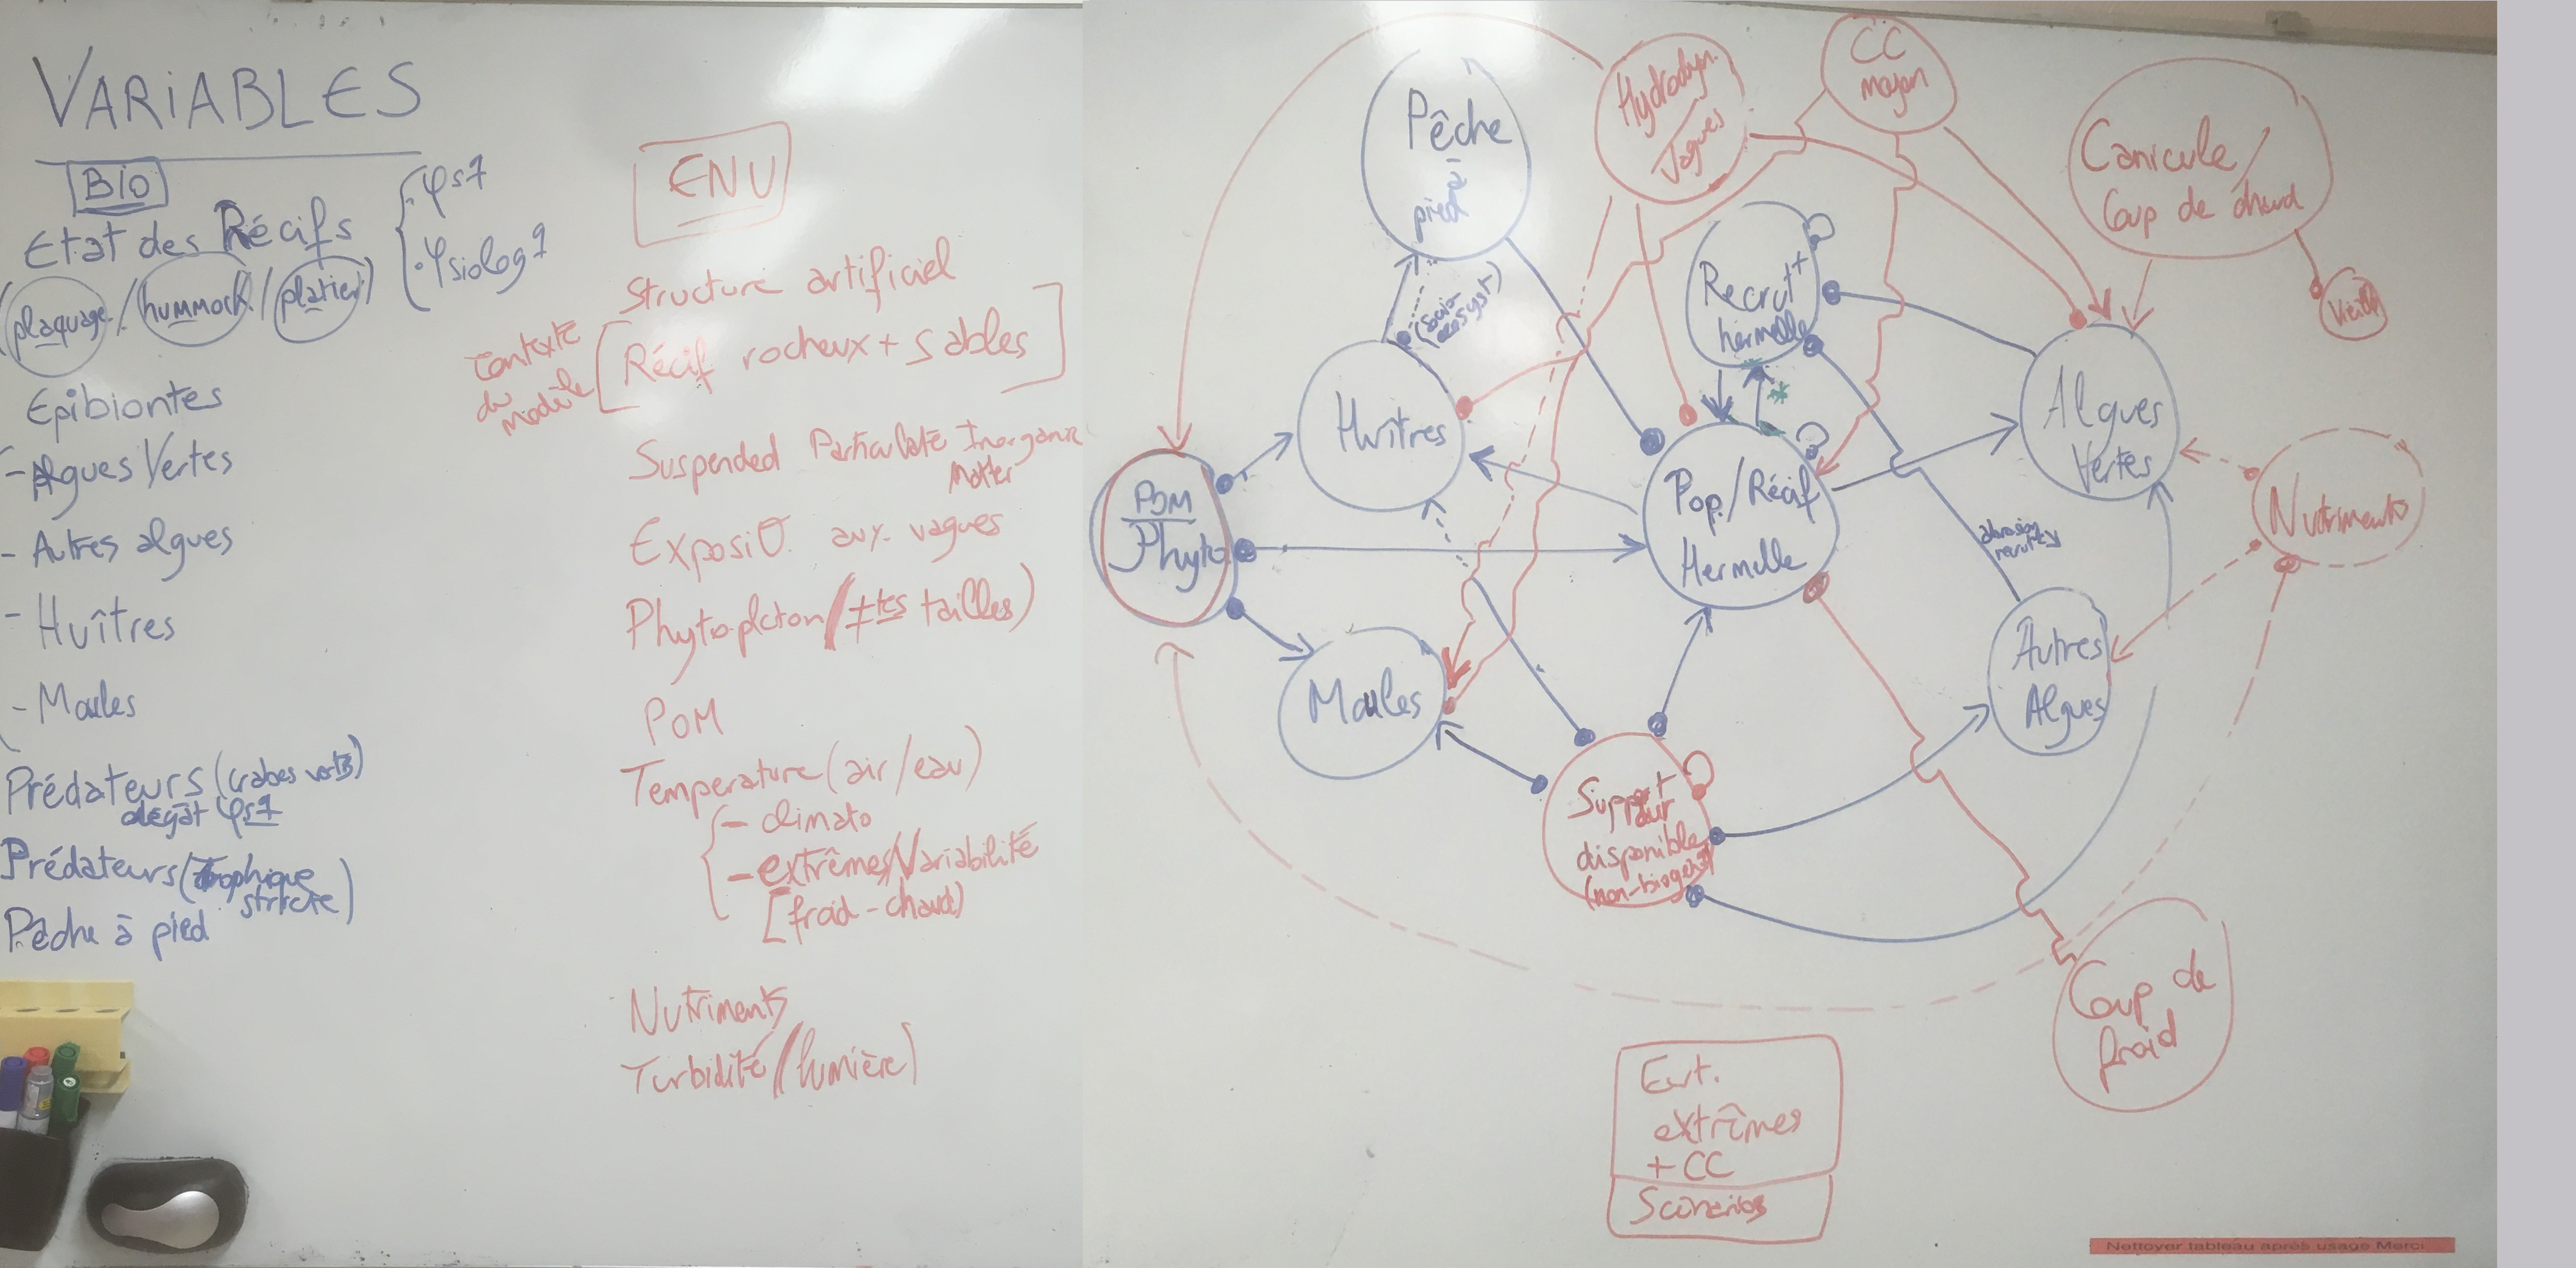
\includegraphics[height = \textwidth, width = .9\textheight,angle = 90]{photo_variables_dessin_merged.jpg}
    \caption[]{Photographie du modèle obtenu après la réunion avec le panel d’experts (model i). Sur la gauche, les variables biotiques et abiotiques à potentiellement intégrer. Sur la droite, le schéma conceptuel du modèle avec les variables et les interactions. Les flèches correspondent à un impact positif sur le nœud d’arrivé et les points noirs représentent un impact négatif.Les relations en pointillés correspondent à des processus secondaire dont l'inclusion dans le modèle est incertaine. }
    % \vspace{-8mm}
    \label{fig:1}
\end{wrapfigure}


\begin{wrapfigure}{r}{}
    \centering
    \includegraphics[height = \textwidth, width = .9\textheight,angle = 90]{reehab_sheet.jpg}
    \caption[]{Feuille standardisée de récoltes de données REEHAB}
    \label{fig:2anx}
\end{wrapfigure}

\begin{wrapfigure}{r}{}
    \centering
    \includegraphics[width = \textwidth, height = .9\textheight]{dia_merged.pdf}
    \caption[]{Liste des modèles explorés avec la méthode des modèles qualitatifs. Les noms sont ceux utilisés lors de nos analyses statistiques. \textbf{a} = Model I (\textit{i.e.} modèle expert tel que pensé pour la première fois), \textbf{b} = Model Algae (rassemblement des noeuds Other Algae et Green Algae), \textbf{c} = Model Competitors (rassemblement des noeuds Oyster et Mussel), \textbf{d} = Model Oyster (rertait du noeud Mussel), \textbf{e} = Model Simple (un seul noeud Competitors et un seul noeud Algae), \textbf{f} = Model Mussel (rertait du neoud Oyster), \textbf{g} = Model I No POM, \textbf{h} = Model Algae No POM (\textit{i.e.} modèle validé \textit{in fine})}
    \label{fig:3anx}
\end{wrapfigure}

\begin{wrapfigure}{r}{}
    \centering
    \includegraphics[height = \textwidth, width = .9\textheight,angle = 90]{boyé_ff.png}
    \caption[]{Graphe des dépendances partielles issues de modèles de Boosted Regression Trees (BRT) prédisant l'occurence des six régimes (a-f) de récifs à \textit{Sabellaria alveolata} définis par Boyé \textit{et al.} (in prep). Les dépendances partielles sont représentées avec leur intervalles de confiance à 95\% issus de bootstrap. Seules les 5 variables les plus influentes dans la construction de chaque modèle sont représentées. L'influence relative de chaque variable dans la construction est reportée entre parenthèse. Les tirets en haut de chaque graphique représentent des points observés dans les données. Pour plus de détails sur l'approche de modélisation de régimes par BRT, se référer à Jouffray\textit{ et al. }, 2017.
}
    \label{fig:4anx}
\end{wrapfigure}

\begin{wrapfigure}{r}{}
    \centering
    \includegraphics[height = \textwidth, width = .9\textheight,angle = 90]{mean_gowdis_sd.jpg}
    \caption[]{Modèle qualitatif Algae No POM validé par nos analyses. L'épaisseur des flèches représente la distance de Gower moyenne au modèle original après retrait de l'interaction pour chaque scénario. C'est une synthèse de la \autoref{fig:6}, qui peut être vu comme représentant la contribution moyenne de chaque interaction dans la réponse du modèle. La partie grisée représente l'écart-type.}
    \label{fig:5anx}
\end{wrapfigure}

\begin{wrapfigure}{r}{}
    \centering
    \includegraphics[height = \textwidth, width = .9\textheight,angle = 90]{all_bn.pdf}
    \caption[]{Réseaux Bayésiens inférés avec différentes méthodes et différents packages. HC = Hill Climbing, MMHC = Max-Min Hill Climbing, SM = Silander-Myllymaki}
    \label{fig:6anx}
\end{wrapfigure}

\cleardoublepage 

\includepdf[page = 1]{abstract_final.pdf}


\end{document}


